%%%%%%%%%%%%%%%%%%%%%%%%%%%%%%%%%%%%%%%%%%%%%%%%%%%%%%%%%%%%%%%%%%% 
%                       rpithes-short.tex                         %
%         Template for a short thesis all in one file             %
%        (titlepage info below assumes masters degree}            %
%  Just run latex (or pdflatex) on this file to see how it looks  %
%      Be sure to run twice to get correct TOC and citations      %
%%%%%%%%%%%%%%%%%%%%%%%%%%%%%%%%%%%%%%%%%%%%%%%%%%%%%%%%%%%%%%%%%%% 
%
%  To produce the abstract title page followed by the abstract,
%  see the template file, "abstitle-mas.tex"
%
%%%%%%%%%%%%%%%%%%%%%%%%%%%%%%%%%%%%%%%%%%%%%%%%%%%%%%%%%%%%%%%%%%%

\documentclass{thesis}
\usepackage{graphicx}
\usepackage{url}
\usepackage{subfig}

% Use the first command below if you want captions over 1 line indented.
% A side effect of this is to remove the use of bold for captions. 
% To restore bold, also include the second line below.
%\usepackage[hang]{caption}     % to indent subsequent lines of captions
\renewcommand{\captionfont}{\bfseries} % only needed with caption package;
                                        %   otherwise bold is default)
%%%%%%%%%%%%%%%%%%%%  supply titlepage info  %%%%%%%%%%%%%%%%%%%%%
\thesistitle{\bf Thin Shell Structure Design Tool}        
\author{R. Allan Pendergrast}
\degree{Master of Science}
\department{Computer Science}
\thadviser{Barbara M. Cutler}
\submitdate{May 2010\\(For Graduation May 2010)}        
%\copyrightyear{1685}  % if date omitted, current year is used. 
%%%%%%%%%%%%%%%%%%%%%   end titlepage info  %%%%%%%%%%%%%%%%%%%%%%
      
\begin{document} 
\titlepage             % Print titlepage   
%\copyrightpage        % optional         
\tableofcontents       % required 
\listoftables          % required if there are tables
\listoffigures         % required if there are figures

\specialhead{ACKNOWLEDGMENT}
Thanks to Barbara Cutler for all her help in creating, testing, and writing about this tool.  Thanks to my family for their endless
support as I worked on this project.  Thanks to the user study subjects for participating in the study and providing me with valuable
insight into what can be done to improve this tool.

\specialhead{ABSTRACT}
Thin-shell structures are becoming increasingly useful in construction and design of buildings.  They allow the usage of less material to enclose
larger spaces, are structurally efficient, and have a natural aesthetic beauty.  However, they can be difficult to design, as the exact shape
required for structural stability depends on the material used, the size of the shell, and other features.  Fortunately, it is possible to simulate
these structures quickly and accurately, allowing architects to concentrate more on their design and less on ensuring that their building is
stable.  The tool described in this thesis simulates thin-shell structures and aids architects in their design and optimization.

\chapter{INTRODUCTION} \label{chp:introduction}

The goal of this project was to create a tool to aid architects in designing thin-shell structures.  Thin-shell structures can be used in
buildings to save materials, create an open space, or simply for the aesthetic of a smoothly curving shell.  In addition to being beautiful
and materials-friendly, thin-shell structures are also incredibly structurally efficient.  Some thin-shell structures feature shells as thin
as 4 centimeters, yet stand up with nearly no required maintenence for many years.  This structural efficiency is one of the most valuable
characteristics of thin-shell structures.

Structural efficiency is a very important element of construction.  With traditional construction methods, this tends not to be an issue, since
the tried-and-true construction conventions will keep a building standing.  Houses, for example, have been built using the same structural
conventions for years and do not require any advanced structural analysis.  Walls are constructed with studs every 16 inches, and the house
stands up.  Even in non-residential structures, the studded or cinder-block walls convention tends to be followed.  However, when creating
buildings that fall outside the norm of studded walls, cinder block construction, and other such traditional methods, more complex analysis
tools are necessary.

Insufficient analysis of the elements used in constructing a building can result in spectacular disasters such as those
detailed and discussed in \underline{Why Buildings Fall Down}\cite{levy92falldown}.  For example, the C.W. Post Dome covering a theatre on the
campus of C.W. Post College collapsed suddenly under a load of snow much lower than the dome had been built to withstand.  While the dome had
stood up under loads much larger than the one under which it collapsed, the uneven loading of this particular load put undue stress on part
of the dome, leading to a localized instability which spread to cause the whole dome to collapse.  Another famous collapsing structure whose
collapse is discussed in the book is the Tacoma Narros Bridge, also known as ``Galloping Gertie".  While this bridge was designed comparably
to other bridges of the time, certain aerodynamic features were not taken into account.  Under windy conditions, the bridge moved up and down,
sometimes as much as several feet.  This turned out to be due to insufficient stiffness in the deck and ultimately led to the bridge's
collapse.

Conversely, if proper care is taken to analyze structures before they are constructed, miracles of architecture can be constructed that stand
up for thousands of years, as some of the building in Mario Salvadori's \underline{Why Buildings Stand Up}\cite{salvadori80standup} have.

%This project was originally conceived as a structural analysis tool that would find highly over- or underloaded members in a structure
%and notify the architect that some force could be diverted towards the less-used member or that the underloaded member could be
%removed.  This redesigning would help to optimize the structure, resulting in a structure that required less material or work to construct.
%Since then, the focus has shifted to the design and optimization of thin shell structures.  These structures, covered in more detail in
%\ref{thinshell}, are used in architecture to conserve materials, funds, or for simply aesthetic reasons.  Unfortunately, thin-shell
%structures have been famously difficult to optimize and construct, sometime requiring a complete overhaul of the structure to fix stability
%problems. This tool attempts to alleviate this difficulty and make the design and optimization of such structures easier and faster for architects.

\section{Thin Shell Structures} \label{thinshell}

\subsection{Overview}
A thin shell structure is a structure which has a small thickness compared to its other dimensions.  While this may seem to be
an obvious definition, the design and construction of these structures can be complicated.  In traditional construction, load-bearing
members are flat, carrying forces straight through themselves.  A simplified 2D representation of the load-bearing elements of a house
can be seen in Figure \ref{fig:house}.  Larger buildings which are constructed using traditional techniques use very similar techniques
as those used in Figure \ref{fig:house}, employing vertical members and cross-pieces to support the weight of the building.  One
consideration for larger buildings is that large rooms will have large unsupported expanses of floor.  Beams which are loaded transversely
in that manner are subjected to bending according to the Euler-Bernoulli equation: \[EI\frac{d^4u}{dx^4}=w(x)\]
If too much force is applied, the beam will buckle, perhaps causing catastrophic failure.  Therefore, beams and other flat structural
elements must have a high second moment of area (have a large dimension parallel to the applied force) in order to ensure that it will not
buckle under load.  Alternately, columns can be installed to effectively shorten the span which the beam is crossing, but depending on the
application, this may not be desirable.

\begin{figure}
\centering
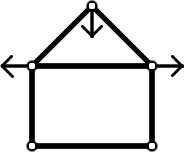
\includegraphics[width=2in]{images/house.png}
\caption[Simplified representation of a house]{This simplified representation of the load-bearing elements of a house show how traditional
construction techniques require additional material to be stable.  Were it not for the horizontal piece which forms the ceiling, the walls
would be forced outward by the forces caused by the weight of the roof.}
\label{fig:house}
\end{figure}

\begin{figure}
\centering
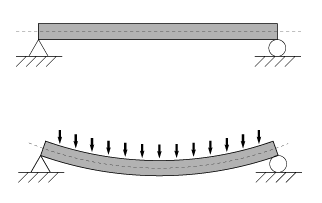
\includegraphics[width=4in]{images/Bending.png}
\caption[A beam under uniform loading]{This is an image of a beam which is deforming under a uniform load.  ``Bending", image created by Daniel De
Leon Martinez, \url+http://en.wikipedia.org/wiki/File:Bending.png+}
\label{fig:bending}
\end{figure}

Unlike normal beam and plate structures, thin shell structures are curved, which allows the force to travel through the thinner structural
elements.  Structures such as those in Figure \ref{fig:isler_service} can cover a large span with a minimal amount of material, saving the
construction company money.  Since the structure completely supports itself, no internal columns are necessary, allowing an unobstructed interior.
An unobstructed interior is very useful in a variety of buildings such as theatres, museums, and airport terminals, to name a few.
Thin-shell structures are very stable because of their unique shape, called a catenary shell.  Catenaries are covered in more detail in Section
\ref{sec:catenary}.  Some prominent thin shell structures include
the TWA Flight Center Building at the JFK International Airport in New York, New York (Fig. \ref{fig:twa_flight}), the Kresge Auditorium on
the MIT campus in Cambridge, Massachusetts (Fig. \ref{fig:kresge_aud}), and the Montreal Biosphere in Montreal, Canada (Fig \ref{fig:montreal_bio}).

\begin{figure}
\centering
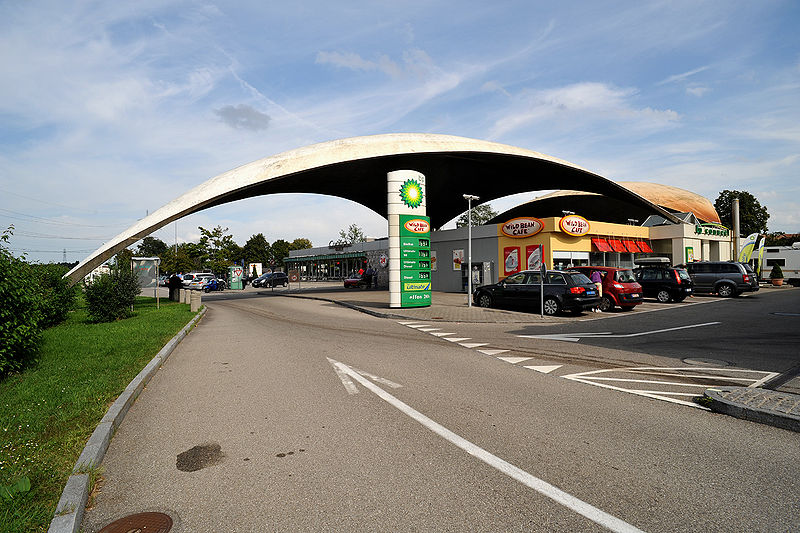
\includegraphics[width=4in]{images/isler_dome_1.jpg}
\caption[A thin-shell dome over a service area in Switzerland]{This dome, designed by Swiss civil engineer Heinz Isler, gracefully arches over
a service station along the A1 Motorway in Switzerland, protecting it from the elements with a minimal amount of material.  ``Deitingen Service
Station"(1968), Heinz Isler, photo taken by Chriusha, \url+http://commons.wikimedia.org/wiki/File:Deitingen_Sued_Raststaette,_Schalendach_04_09.jpg+}
\label{fig:isler_service}
\end{figure}

\begin{figure}
\centering
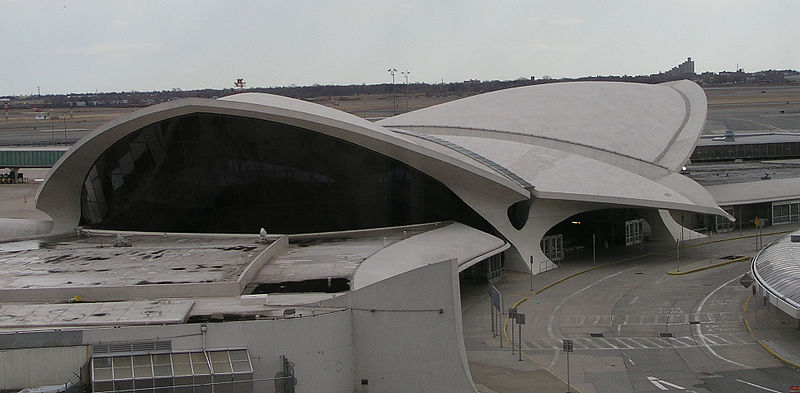
\includegraphics[width=5in]{images/twa_flight_center.jpg}
\caption[The TWA Flight Center]{The TWA Flight Center at JFK International Airport in New York, New York is an excellent modern example of
thin-shell structures providing a much-needed unobstructed internal space.  ``TWA Flight Center", Eero Saarinen, photo taken by Marc N. Weissman
\url+http://en.wikipedia.org/wiki/File:08terminal5.jpg+}
\label{fig:twa_flight}
\end{figure}

\begin{figure}
\centering
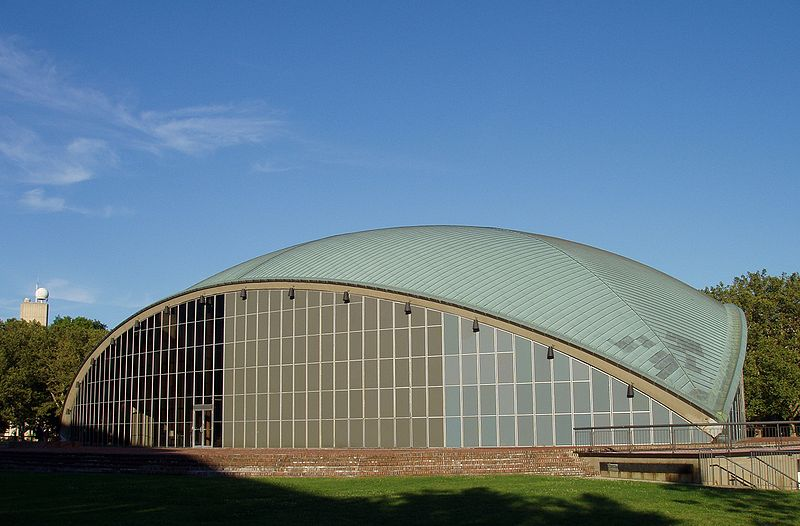
\includegraphics[width=4in]{images/kresge_auditorium.jpg}
\caption[The Kresge Auditorium]{The Kresge Auditorium on the MIT campus in Cambridge, Massachusetts is an example of the problem thin-shell
structures can cause when not designed properly.  Since the roof is octanispherical rather than a catenary shell, the forces do not travel as
intended and the building has been plagued with structural problems since its construction.  ``Kresge Autidorium", Eero Saarinen, photo
taken by Ibn Battuta \url+http://en.wikipedia.org/wiki/File:Kresge_Auditorium,_MIT_(view_with_Green_Building).JPG+}
\label{fig:kresge_aud}
\end{figure}

\begin{figure}
\centering
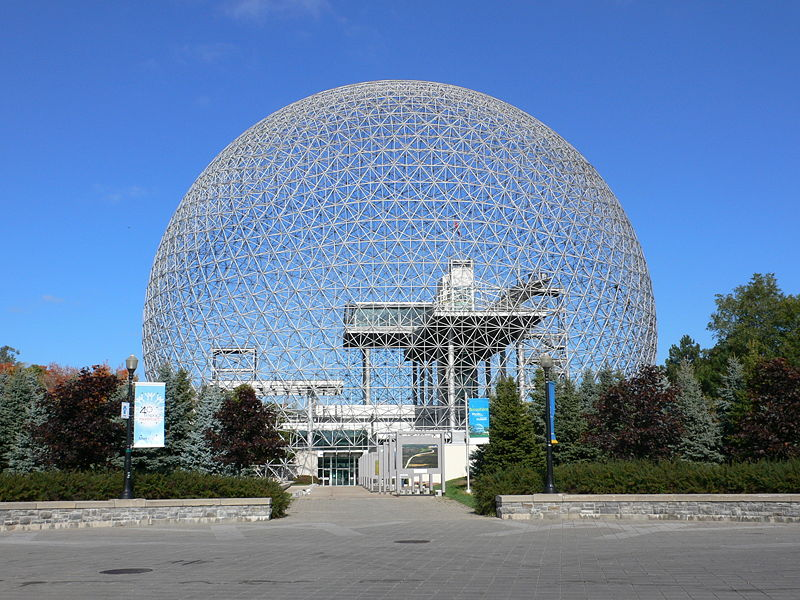
\includegraphics[width=4in]{images/montreal_biosphere.jpg}
\caption[The Montreal Biosphere]{The Montreal Biosphere is an example of a lattice-based thin-shell structure, which relies on a lattice of
struts to support the huge expanse of the dome.  ``Montreal Biosphere", Richard Buckminster Fuller, photo taken by Philipp Hienstorfer
\url+http://en.wikipedia.org/wiki/File:Biosphere_montreal.JPG+}
\label{fig:montreal_bio}
\end{figure}


\subsection{Structural Stability} \label{sec:stability}
The core concept for structural stability for masonry buildings is the concept of lines of thrust.  Lines of thrust are lines that can be drawn
in the direction of the forces neighboring elements of the structure impart on one another.  If all the discrete forces are connected together
into a generalized curve, the traditional lines of thrust are obtained.
In order for a building to stand up, these lines of thrust must pass through structural elements.  As can be seen in Figure \ref{fig:arch_lines},
traditional arches must be rather thick to contain the lines of thrust produced by their weight.  However, a catenary arch can be built
much thinner for the same stability, as it contains the line of thrust exactly.  For example, the Gateway Arch in St. Louis, Missouri (Figure
\ref{fig:gateway_arch}) is constructed in the shape of a catenary arch.  This allows it to be thin and elegant while remaining very stable.
To extrapolate the concept of lines of thrust to entire buildings, traditional construction methods require very thick elements such as walls
and columns to be used in order to keep the lines of thrust within a building's structural elements.  This is especially true of large masonry
structures such as cathedrals.  However, if the shape of the building is instead matched to the shape of the lines of thrust, the structural
elements can be much thinner, since they only need to support the direct compressive force.  Alternatively, if the structural members can
withstand tensile forces, the lines of thrust can be allowed to pass outside the structure, since the resulting tensile forces can be
supported.

\begin{figure}
\centering
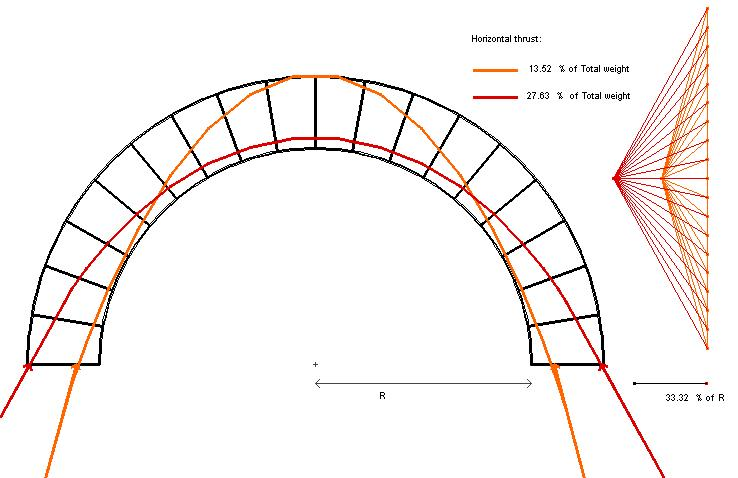
\includegraphics[width=4in]{images/arch.png}
\caption[Lines of thrust]{This figure shows the lines of thrust within a standard masonry arch.  As can be seen from the minimum and maximum
lines, the arch must be rather thick in order to contain the lines of thrust, thereby wasting material.  This image is a screenshot of the
"Interactive Thrust" tool created by Philippe Block.  It can be found at \url+http://web.mit.edu/masonry/interactiveThrust/applets/applet01.html+}
\label{fig:arch_lines}
\end{figure}

\begin{figure}
\centering

\includegraphics[height=3.5in]{images/gateway_arch.jpg}
\caption[The Gateway Arch]{The Gateway Arch in St. Louis, Missouri is an example of a catenary arch.  Since the lines of thrust travel directly
through the structure of the arch, it can be built very thin.  ``Gateway Arch", Eero Saarinen, photo taken by David K. Staub
\url+http://en.wikipedia.org/wiki/File:Gateway_Arch.jpg+}
\label{fig:gateway_arch}
\end{figure}

\subsection{Catenary} \label{sec:catenary}
The term for the shape that lines of thrust take under uniform loading is called a catenary.  A catenary is a curve described by the function
\[y=a cosh\left(\frac{x}{a}\right)\]
where cosh is the hyperbolic cosine function.  Several examples of catenaries can be seen in Figure \ref{fig:catenary}.  In addition to being
an interesting mathematical figure, the catenary is the shape taken by a cable, rope, or chain suspended at both ends, as seen in Figure
\ref{fig:hanging_chain}.  Since this is the shape formed by a freely hanging object under pure tension, it is not surprising that if inverted,
it is similarly stable under pure compression.  For this reason, catenary arches and catenary shells are the primary building blocks of
thin-shell structures.  One very important thing to note is that a catenary is only the optimal shape when the chain or arch is evenly loaded.
If there is an uneven load, for example if the arch has a decorative mass at some point or if a secondary arch rests on another arch, the
catenary is not the optimal shape, as seen in Figure \ref{fig:compound_catenary}.  Furthermore, if the weights are spaced evenly by
horizontal distance rather than by distance on the chain, the chain will form a parabola rather than a catenary.

\begin{figure}
\centering
\subfloat[]{
  \label{fig:catenary}
  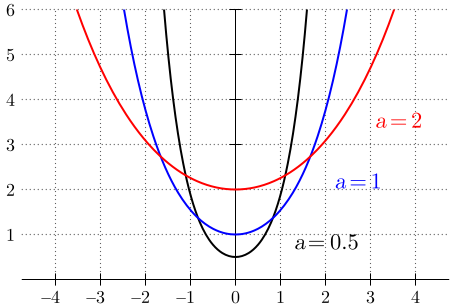
\includegraphics[height=1.7in]{images/catenary.png}
}
\subfloat[]{
  \label{fig:hanging_chain}
  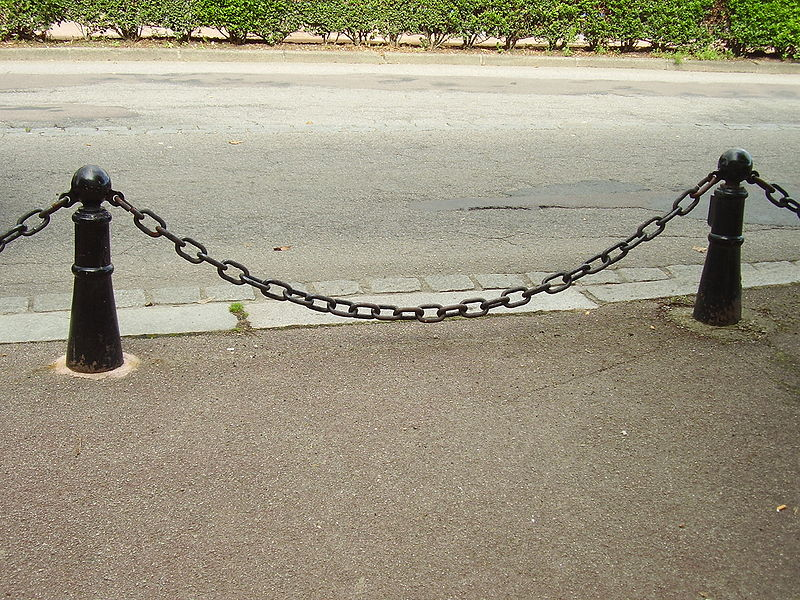
\includegraphics[height=1.7in]{images/hanging_chain.jpg}
}
\caption[Example catenary curves]{Image (a) shows a few catenary curves for various values of a.  ``Catenary Curves", image created
by Geek3, \url+http://en.wikipedia.org/wiki/File:Catenary-pm.svg+  Image (b) shows a natural catenary formed by a freely hanging chain.
"Hanging Chain", photo taken by Kamel15, \url+http://en.wikipedia.org/wiki/File:Kette_Kettenkurve_Catenary_2008_PD.JPG+}
\end{figure}

\begin{figure}
\centering
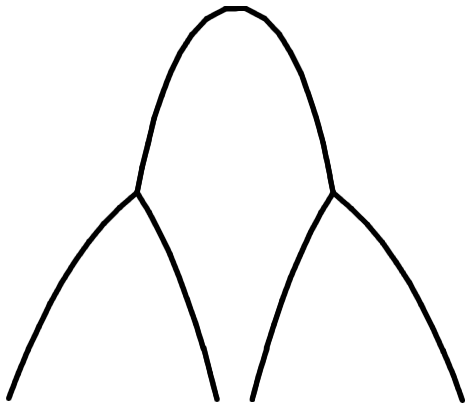
\includegraphics[width=2.25in]{images/compound_catenary.png}
\caption[A composite catenary structure]{This image shows the necessary deformation of supporting catenary arches when a third arch is placed
on top of them.}
\label{fig:compound_catenary}
\end{figure}

The shape of the catenary has been used by many architects.  One example mentioned earlier is the Gateway Arch in St. Louis, Missouri, designed by
the Finnish-American architect Eero Saarinen and seen in Figure \ref{fig:gateway_arch}.  However, the shape has also been used as an integral design
principle for much larger and more complex structures.  Hanging chains have been used by a number of architects to design structures for stability and
aesthetics.  One famous user of hanging chains is Antoni Gaud\'{i}, whose catenary-rich projects include such Barcelona landmarks as the Casa Mil\`{a}
(Figure \ref{fig:casa_mila}), Park Guell (Figure \ref{fig:parc_guell}), and Sagrada Familia (Figure \ref{fig:sagrada_familia}).  The works of Antoni
Gaud\'{i}, his design methods, and his aesthetic style are beautifully photographed, discussed, and analyzed in Rainer Zerbst's
\underline{Antoni Gaud\'{i} The Complete Buildings}\cite{zerbst85gaudi}.  Figure \ref{fig:gaudi_model} shows one of the models Gaud\'{i} used in
creating these graceful structures.

\begin{figure}
\centering
\subfloat[]{
	\label{fig:casa_mila_ext}
	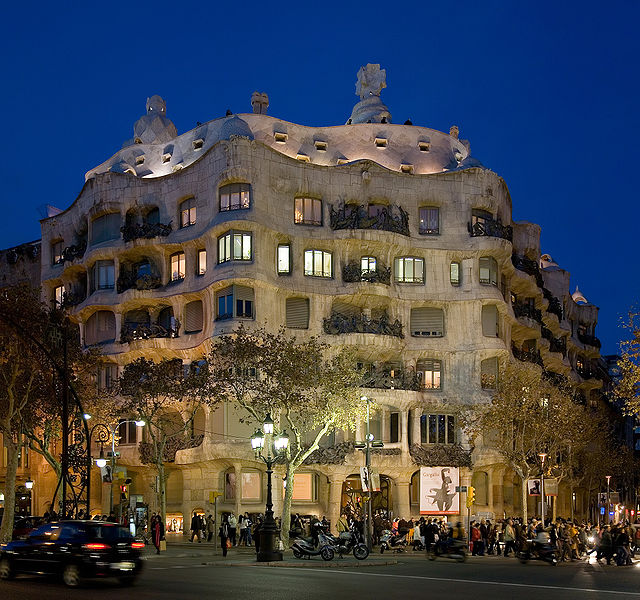
\includegraphics[height=3in]{images/casa_mila_ext.jpg}
}
\subfloat[]{
	\label{fig:casa_mila_arch}
	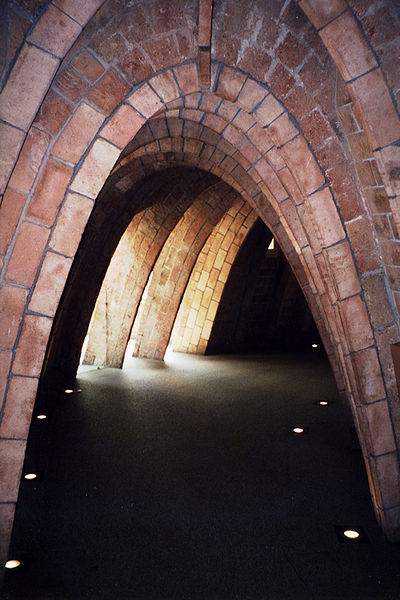
\includegraphics[height=3in]{images/casa_mila_arch.jpg}
}
\caption[Casa Mil\`{a}, Barcelona, Spain]{Image (a) shows an exterior view of Casa Mil\`{a}, one of Antoni Gaud\'{i}'s stunning buildings in
Barcelona, Spain. ``Casa Mil\`{a}", Antoni Gaud\'{i}, photo taken by David Iliff
\url+http://en.wikipedia.org/wiki/File:Casa_Mil\`{a}_-_Barcelona,_Spain_-_Jan_2007.jpg+ Image (b) is of the catenary arches under the terrace
of Casa Mil\`{a}. ``Casa Mil\`{a}", Antoni Gaud\'{i}, photo taken by Error, \url+http://en.wikipedia.org/wiki/File:LaPedreraParabola.jpg+}
\label{fig:casa_mila}
\end{figure}

\begin{figure}
\centering
\subfloat[]{
	\label{fig:parc_guell_ent}
	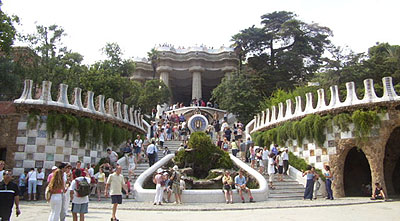
\includegraphics[height=2in]{images/parc_guell.jpg}
}
\subfloat[]{
	\label{fig:parc_guell_arch}
	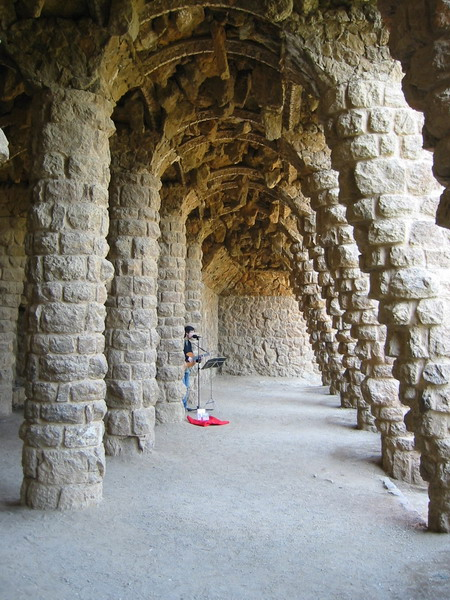
\includegraphics[height=2in]{images/parc_guell_arch.jpg}
}
\caption[Parc Guell, Barcelona, Spain]{Image (a) shows the entrance to Parc Guell in Barcelona.  ``Parc Guell Entrance", Antoni Gaud\'{i}, photo
taken by Montrealais \url+http://en.wikipedia.org/wiki/File:Parcguell.jpg+  Image (b) shows the columns supporting the roadway that runs past the
park.  These columns form an offset catenary, which is asymmetric because the loading of the arch is asymmetric. ``Parc Guell", Antoni Gaud\'{i},
photo taken by Rapomon, \url+http://en.wikipedia.org/wiki/File:Parc_Guell_10.jpg+}
\label{fig:parc_guell}
\end{figure}

\begin{figure}
\centering
\subfloat[]{
	\label{fig:sagrada_familia_nativity}
	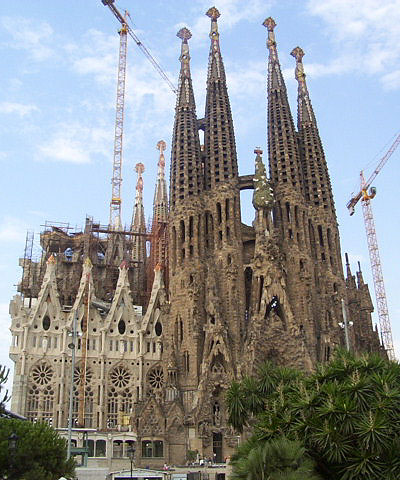
\includegraphics[width=2.5in]{images/sagrada_familia_nativity.jpg}
}
\subfloat[]{
	\label{fig:sagrada_familia_columns}
	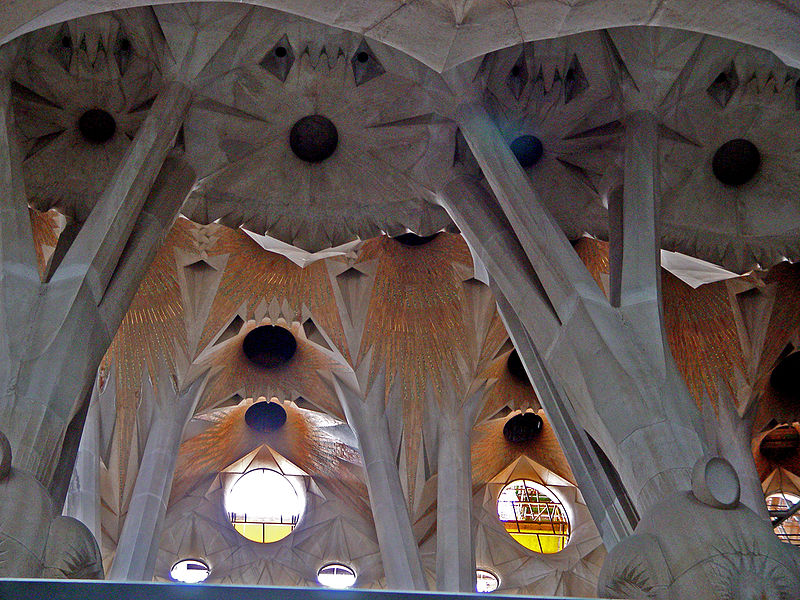
\includegraphics[width=3in]{images/sagrada_familia_columns.jpg}
}
\caption[Sagrada Fam\'{i}lia, Barcelona, Spain]{Image (a) shows the nativity fa\c{c}ade of Antoni Gad\'{i}'s masterpiece, Sagrada Fam\'{i}lia,
slated to be completed some time after 2026.  ``Sagrada Fam\'{i}lia", Antoni Gaud\'{i}, photo taken by Montrealais,
\url+http://en.wikipedia.org/wiki/File:Sagradafamilia-overview.jpg+  Image (b) shows the strucutral columns that are possible when
designing with catenaries in mind.  Rather than the monolithic columns found in most gothic cathedrals, Gaud\'{i} has whittled away the nonessential
stone to reveal the core load-bearing elements.  This results in a gracefully arcing column that supports the huge structure as well as a monolithic
column would have.  ``Sagrada Fami\'{i}lia", Antoni Gaud\'{i}, photo taken by Etan J. Tal,
\url+http://en.wikipedia.org/wiki/File:SagradaFamiliaRoof.jpg+}
\label{fig:sagrada_familia}
\end{figure}

\begin{figure}
\centering
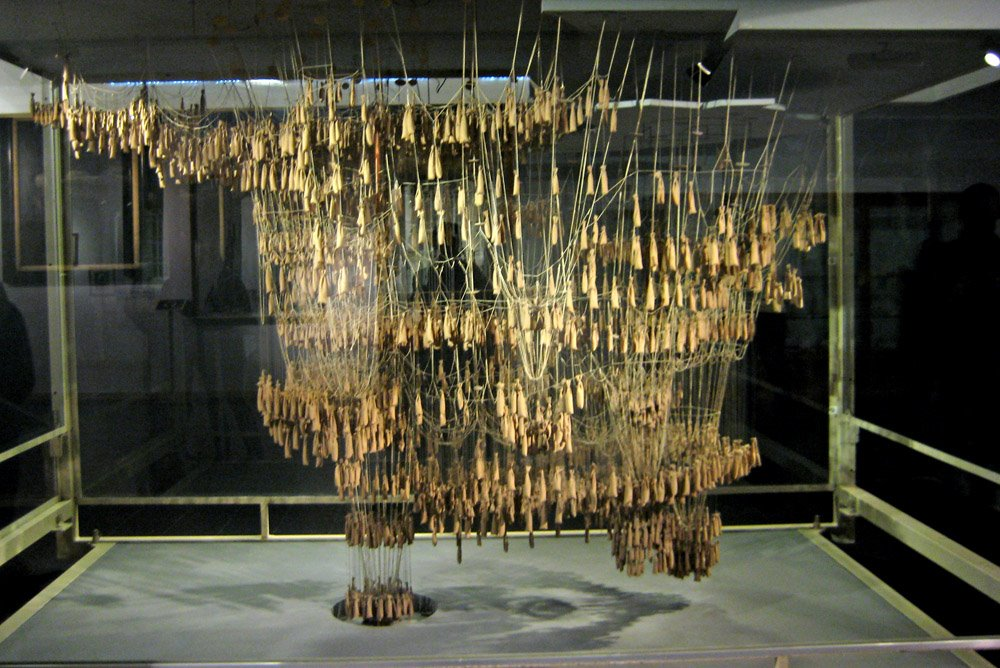
\includegraphics[width=4in]{images/gaudi_model.jpg}
\caption[A hanging model used by Gaud\'{i}]{This is a photo of one of the hanging models used by Antoni Gaud\'{i} to understand the forces in
the buildings he constructed.  The bags are full of small lead weights which are proportonal to various structural elements and ornaments in
the planned building.  The strings holding them together are the necessary columns, arches, and other core structural elements that will make
up the building.  ``Hanging model", Antoni Gaud\'{i}, photo taken by Pamela Angus, 
\url*http://2.bp.blogspot.com/_PZOVPTsrTJ0/SR7z2F_h93I/AAAAAAAAAls/hAv1--bslzQ/s1600-h/Gaudi+model.jpg*}
\label{fig:gaudi_model}
\end{figure}

Another architect who is well-known for his use of thin shells in his structures is Heinz Isler.  A civil engineer from Switzerland,
Isler designed some very beautiful and elegant structures using the simple tools of cloth and water.  Since a sheet of cloth will behave as an
interconnected set of hanging strings, it can be used to create catenary shell structures.  What Isler did was to take the shape a sheet of cloth
formed when suspended and freeze it by soaking the cloth evenly with water.  The resulting frozen structure was then inverted and measured very
accurately with a device he created.  Once these measurements had been taken, he built forms and poured the shell using standard concrete
construction techniques.  The resulting buildings, such as those in Figure \ref{fig:isler_service}, are elegant, graceful structures with an
exquisite simplicity of form and conservation of material.  In 1997, he gave a lecture in honor of F\'{e}lix Candela\cite{isler97candela} in
which he discussed his design process and inspiration in great detail.

One drawback to the thin-shell structure work done by Gaud\'{i} and Isler is that the design process is very time-consuming.  The amount of time
it takes to create a hanging model from strings and lead shot or freeze a cloth shell is prohibitive to the fast-paced, quick turnaround time of
the modern architecture world.  Fortunately, both hanging chains and cloth are rather easy to simulate, and therefore software can be created to
allow these designs to be rapidly prototyped, tweaked, and refined on the computer.

\section{Overview}
In chapter two, I will discuss a number of related works and their influence on this project.  Papers on
procedural structure generation and cloth simulation are discussed, along with structural analysis sofware.
Chapter three contains a description of the simulation algorithm used in this tool.  Advantages and
disadvantages of various simulation methods are discussed, and the algorithm selected is described in detail.
Chapter four concerns the design of the user interface.  The various elements of the interface, as well as
features that are not evident from screenshots of the tool are discussed in this chapter.  Chapter five is
about the user study.  The design considerations when putting the study together are discussed, as well as
responses recieved from the users.  In addition, observations of the users are included.  These observations
provided some of the most relevant information about the tool that I obtained from the study.  Chapter six
contains discussions on future work.  There are many things that could be changed about this tool, and most
of these potential changes are detailed in this section.  Chapter seven contains some conclusions about the
process.

\clearpage
\chapter{RELATED WORKS}
\section{Procedural Modeling}
In ``Procedural Modeling of Strucutrally-Sound Masonry Buildings"\cite{whiting:2009}, Whiting, Ochsendorf, and Durand explore
the possibilities of creating existing or novel structures procedurally.  They began by creating a grammar
which can be used to construct masonry buildings.  Arches, buttresses, domes, and vaults are some of the
structural elements which are then combined in their software.  These grammar elements are assembled into
a structure through a procedural algorithm which cuts windows in walls and assembles
all the various masonry elements of the building.  Once the initial configuration is
generated, the software runs static analysis on the building.  If it is feasibly stable, the program is
done.  If not, the program determines a measure of infeasibility, which is a measure of how far away from
stable a structure is.  The static analysis only allows for compressive forces, as the tensile strength of
masonry elements is close to zero.  Friction is also modeled, allowing for some shear.  Once the measure
of infeasibility is calculated, a parameter search is conducted iteratively, searching the parameter space
for a stable configuration.  Depending on the application, this stable configuration will take into account
a factor of safety.  The more likely a structure is to have changing loads, the higher a factor of
safety is needed.  For example, a bridge needs a higher factor of safety than a cathedral.  In the event
that there is no feasible configuration for a structure, the least infeasible structure is returned and the
user is required to add new structural elements.

In ``Creating Models of Truss Structures with Optimization"\cite{Carnegie02creatingmodels}, Smith, Hodgins, Oppenheim, and Witkin propose
a method of creating trusses procedurally.  This work allows the user to define several anchor points
and loads for a truss, then have the software automatically generate a truss.  In this work, the risk
of pieces falling apart is not an issue as it was in the previous paper.  The primary failure method
in this case is buckling, since all forces are axial.  Therefore, the core of the algorithm is a
multivariable optimization with constraints.  The algorithm attempts iteratively to minimize weight
while ensuring that none of the members will fail, either in tension or compression.

My work had initially intended to go in this direction, using static analysis of structures within
Google SketchUp.  However, SketchUp proved to be a poor environment for the program I wanted to write, so
the project was moved to a standalone application and the focus shifted to thin-shell structures.  With this
shift in focus, the simulation method shifted from static analysis of structures to dynamic simulation of
structure using techniques from cloth simulation.  This simulation was designed to imitate the behavior of
hanging chains or cloth.

Hanging chains and cloth have been used by a number of architects in the design of structures.  In
\underline{Finding Form}\cite{otto95findingform}, Frei Otto and Bodo Rasch discuss a number of natural inspirations of form, among which
is hanging chains.  They show that a naturally hanging square-mesh chain net will form the shape of
traditional Asian roofs, while inverting chain nets suspended differently will yield the ideal structure
for arches, domes, and vaults.  While this has been known for some time, it is comforting to see
well-documented, carefully constructed pictures of these structures.  As was discussed in \ref{sec:catenary},
Antoni Gaud\'{i} and Heinz Isler used thin-shell structures and hanging chains similar to those described in
\underline{Finding Form} constantly as an integral part of their design processes.
\nocite{charleson05structasarch}

\section{Cloth Simulation}
Much work has been done in the field of cloth simulation.  In ``The Synthesis of Cloth
Objects"\cite{weil86synthcloth}, Jerry Weil lays the groundwork for much of the future of cloth simulation.
Weil describes a method of surface generation that draws catenaries between points in order to approximate
the surface of a hanging cloth, then iteratively relaxes the surface to more accurately represent a
naturally draping piece of cloth.

Further work on the simulation of elastic bodies was done by Terzopoulos, Platt, Barr, and Fleischer in
"Elastically Deformable Models"\cite{terzopoulos87elastic}.  This paper yields results that are applicable
much more generally than simply cloth simulation.  The elastic model that is created can be used for cloth,
solids, and other elastic manifolds.  By summing the internal strain energies and energies applied by
external forces such as gravity or wind then integrating the resulting equations numerically, an animation
of these deformable models can be created.

These early examples of cloth simulation are expanded upon by Volino, Courchesne, and Thalmann in ``Versatile
and efficient techniques for simulating cloth and other deformable objects"\cite{volino95cloth}.  In this
paper, the internal shear and bending strain energies and external forces are augmented by further collision
energies, such as self-collision.  This algorithm is robust enough to simulate such complex situations as
cloth tumbling in a dryer and a dress draping around a walking human.

In ``Deformation constraints in a mass-spring model to describe rigid cloth behavior"\cite{provot95deformationconstraints},
Xavier Provot describes a method for cloth simulation on which the simulation used in this thesis is based.
A cloth consisting of a mesh of masses and springs is subjected to external forces such as gravity.  These
external forces are combined with internal spring forces to obtain the total force on each point.  However,
this simulation method results in overstretching, the cloth behaving more like putty than cloth.  Therefore,
Provot implements a correction step, wherein the points are brought closer together if they have stretched
farther than some allowed amount.  This correction prevents the cloth from stretching farther than reality
would allow.

Far more advanced cloth simulation methods have been developed more recently which are not implemented in
this project but which are planned for future work.  In ``Large Steps in Cloth Simulation"\cite{baraff98largesteps},
Baraff and Witkin propose an implicit simulation method which is the basis for most modern cloth simulation.
The same shear and bending forces used in the earlier methods, as well as gravity and other external forces
are applied to the cloth, but instead of being explicitly integrated, an implicit integration method employing
sparse matrices is employed.  The sparse matrix of equations resulting from the internal and external forces
is solved using a modified Conjugate Gradients method that can operate on asymmetric systems.

\section{Other Software}
There is a large variety of software available for structural analysis, architectural modeling, and even
catenary design.

Foremost in the field of finite element analysis is NASTRAN\cite{NASTRAN}.  Originally developed for NASA in
the 1960s, NASTRAN is one of the most advanced finite element analysis packages on the market.  Able to
analyze both static and dynamic systems in a wide variety of failure modes, NASTRAN is the software
of choice for analysis of parts and systems for any mechanical application.  While NASTRAN is very good
at what it does, it gives information on a lower level than is relevant for most architectural applications.
Furthermore, it is not a real-time application.

Another piece of software that is relevant in architectural design is Dr. Frame 3D\cite{drframe}.  This
software is more useful in architectural design than NASTRAN, as there is an interface for building frames and structures.
Once constructed, the user can apply loads and see the resulting deformations, moments, and other relevant
visualizations.  However, as with standard architectural CAD packages such as Rhino\cite{rhino} and
AutoCAD Architecture\cite{autocad}, it is tedious to construct an accurate catenary, as there are no
tools for easily creating an arbitrary stable shell.

One tool that is useful in creating arbitrary shell structures is CADenary\cite{cadenary}.  With this tool,
users can attach endpoints of strings and sheets to points on a grid or points on existing strings and sheets.
Interesting shells can be made, but once points are placed they are fixed, which is disadvantageous for
iterative design.  In his paper ``Linking Hanging Chain Models to Fabrication"\cite{kilian05cadenary}, Axel Kilian
discusses his tool in finer detail, detailing its features and the design process behind it.


\chapter{SIMULATION ALGORITHM}
Armed with the knowledge gained from these previous works, I set out to create a back end that would accurately
and quickly find the stable configurations of various thin-shell structures.  Algorithms from cloth simulation,
concepts from procedural modeling, and design ideas from similar software were combined to create the backend for
this tool.  In this section, I will discuss the data structures used to implement this tool as well as algorithms
that are applied to the data structures.  A discussion on the advantages and disadvantages of the selected algorithm
is also included.

\section{Data Structure}
The primary data structure is the cloth object.  This object contains an array of points which are connected to each other through springs.
Each point has a list of structural and shear springs that are connected to it.  These springs know what their resting length is and have
a pointer to the point at the other end.  These springs exert forces on the points to which they are connected based on stiffness constants
which are determined when the cloth is loaded.  The other attribute that points can have is the ``fixed" attribute.  Fixed points are
attached to the ground and can be moved only by the user manipulating the points in the floorplan pane.

This data structure taken as a whole represents a discrete mesh, upon which a simulation can be run.  Figure \ref{fig:wireframe} shows
the wireframe view of a model within the simulator.  The lines in the image are the springs connecting points, and each place where
the points meet is a discrete mass.  Each point has both structural and shear springs coming from it, and the forces applied by these
springs together with the force of gravity give the shell its stable shape.  In Figure \ref{fig:wireframe_detail}, the forces acting on
a point are annotated.  The green arrow represents gravity, the red arrows mark the structural springs, and the blue arrows mark the
shear springs.  It may seem curious that gravity is applying a force in the upward direction, but the reason for this is to make the
structure easier to comprehend.  While the simulator is constructing a hanging chain model, the architect is interested in the final
shell, which is the hanging chain model inverted.  Therefore, since this is a simulator, gravity can easily be inverted within the
simulation to obtain accurate results in an easily visualized form.  The structural forces are the hanging chains in the simulation,
connecting the discrete masses together.  The shear forces are the forces that would be exerted by the actual material were it
continuous rather than consisting of discretized masses.

\begin{figure}
\centering
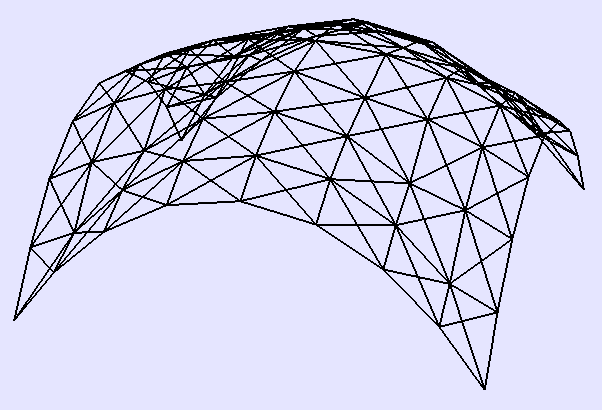
\includegraphics[width=3in]{images/wireframe.png}
\caption[A wireframe of a simulated model]{This image shows a wireframe in the simulator.  The lines represent springs, while the points
where they meet are the discrete points of mass.  The points at the corners have been fixed, which means that they must support the weight
of the entire shell.  These points are not affected by the simulation, and can only be moved by the user.}
\label{fig:wireframe}
\end{figure}

\begin{figure}
\centering
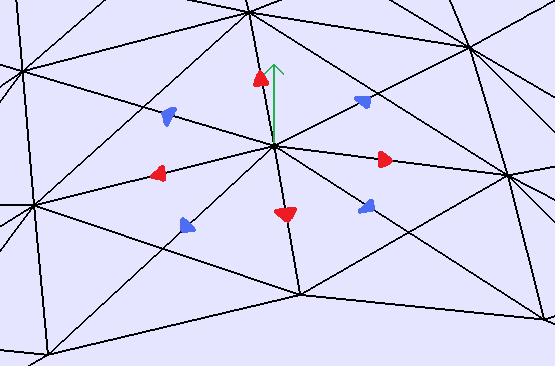
\includegraphics[width=3in]{images/wireframe_detail.png}
\caption[Detail of a wireframe of a simulated model]{This image shows annotations on a portion of a wireframe.  In this image, the black
vertical arrow is the gravitational force, the red orthogonal arrows are the structural forces, and the light blue diagonal arrows are the
shear forces.}
\label{fig:wireframe_detail}
\end{figure}

\section{Algorithm}
The algorithm which was to be applied to this cloth structure needed to be quick enough to maintain a high framerate, but robust enough
that reasonable timesteps could be taken in order to reach an equilibrium where all the forces cancel each other out quickly.
Furthermore, it needed to be able to find an equilibrium without becoming unstable and degenerating into a chaotic mess.  The
best candidate for an integration method that met all of these criteria is a second-order explicit Euler integration.  This
integration method is also called the Midpoint method.

The implementation of the Midpoint method is rather straightforward, and is an expansion of the first order explicit Euler integration
method.  First order explicit Euler integration finds the tangent line of the function at the current point, then moves in that direction
for a timestep and repeats.  Therefore, at each step of the simulation, the system iterates over all the vertices in the shell, and for
each vertex calculates the forces acting upon it.  As shown in Figure \ref{fig:wireframe_detail}, the forces acting upon any given point are
gravity and the spring force exerted by all connected points.  The total force can therefore be calculated as \[F_g+\sum{F_{si}}\]
Where $F_g$ is the force of gravity and $F_{si}$ are the spring forces acting on the point.

Once the total forces have been calculated, the algorithm divides the forces by the masses of the points, yielding an acceleration.
The acceleration can by multiplied by the time step to obtain a velocity, which is again multiplied by the time step to get the new
position of the point: $a=\frac{F}{m}$, $v=a\times t$, $x=v\times t$.
However, this single-step explicit integration is very imprecise.  If the timestep or forces involved are very large, the result will
have a large amount of error, which can cause instability, inaccuracy, or oscillation.  Figure \ref{fig:euler_integration} shows the
inaccuracies that can develop when trying to approximate a function with first-order Euler integration.

To alleviate this problem, rather than taking a step using the forces calculated at the initial point, a half step is taken instead.
Once this half step has been taken, the forces are re-calculated and a full step is taken from the initial point using these new forces.
The end result is that a step is taken from the inital point in approximately the direction of the tangent line of the force function at
the midpoint of the step. This second-order integration method is much more stable, so much larger timesteps can be taken with comparable
accuracy, as shown in Figure \ref{fig:euler_integration}.

A fourth-order Runge-Kutta system was created, but despite its stability, each step took too long for it to be useful in an interactive
simulation.  The fourth-order Runge-Kutta method, commonly referred to simply as \emph{the} Runge-Kutta method, was developed around 1900
by Runge and Kutta.  It can be expanded to any order, but the fourth-order version is the most commonly used.  In order to take a step
using the Runge-Kutta method, four slopes must be calculated.  $k_1$ is the slope at the inital point, $k_2$ is the slope at the midpoint,
calculated using $k_1$ as the slope from the inial point, $k_3$ is the slope at the midpoint calculated using $k_2$ as the slope from the
inital point, and $k_4$ is the slope at the end of the step, calculated using $k_3$ as the slope from the inial point.  The final slope
is then calculated as \[slope=\frac{1}{6}(k_1+2k_2+2k_3+k_4)\]  A step is then taken in the direction specified by this final slope.

\begin{figure}
\centering
\subfloat[]{
	\label{fig:euler1}
	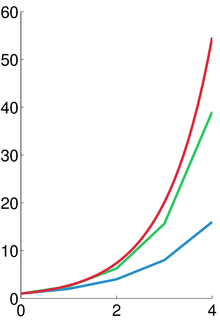
\includegraphics[width=2in]{images/euler1.png}
}
\subfloat[]{
	\label{fig:euler.25}
	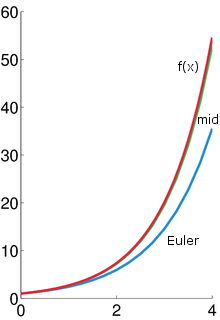
\includegraphics[width=2in]{images/euler25.png}
}
\caption[Euler integration]{These images show the error that is present in explicit Euler integration.  The red line is the target
function f(x), the blue line is first order Euler integration, and the green line is the midpoint method.  Image (a) has a timestep of 1,
while image (b) has a timestep of 0.25.  As can be seen, the smaller timestep results in lower error, but error is still present.
In (b), the target function and midpoint method lines are nearly indistinguishable, showing the accuracy of the midpoint method with
proper timestep selection.}
\label{fig:euler_integration}
\end{figure}

After the Euler integration is performed, overstretched springs are shortened in two ways.  First, the saved original length of the
spring is shortened so that the force pulling it back towards the original shape will be higher.  This correction will reverse and
increase the original length if the overstretched spring becomes overcontracted.  Secondly, the points will be adjusted such that
a hard cap is enforced on the lengths of the springs in order to prevent the deformation from becoming too severe, as detailed
in\cite{provot95deformationconstraints}.  While a higher spring constant would also cause the springs to stay shorter in general,
if the constant becomes too large, the forces within the cloth will become very large and the simulation will become
unstable.  The only way to combat an unstable simulation using the Midpoint method is by shrinking the timestep, which
will slow down the simulation.  In order for the simulation to be interactive, a large enough timestep must be used that a stiff
cloth is not feasible, thus requiring the use of these correction techniques.

This simulation finds equilibrium when the forces exerted by the springs balance the force of gravity and the velocities of the particles
are all zero.  Depending on the number of points in the shell and the changes made to the shape since it was last in equilibrium, the
simulation could take anywhere from a few seconds to a few minutes to reach this resting state.  Figure \ref{fig:wireframe_sim} shows
the motion of a shell as it progresses from an initial mesh to a stable thin-shell configuration.

\begin{figure}
\centering
\subfloat[]{
	\label{fig:wireframe_sim1}
	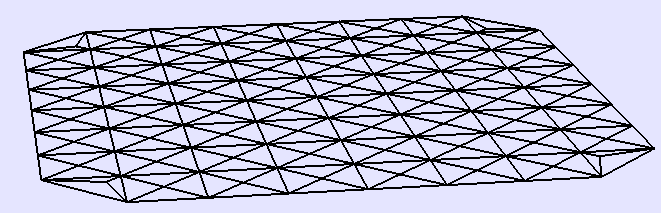
\includegraphics[width=3in]{images/simframe1.png}
}
\subfloat[]{
	\label{fig:wireframe_sim2}
	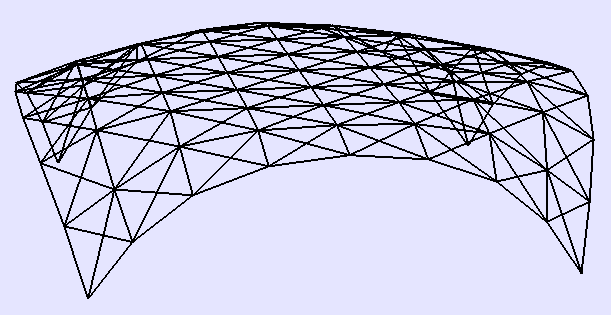
\includegraphics[width=3in]{images/simframe2.png}
}\\
\subfloat[]{
	\label{fig:wireframe_sim3}
	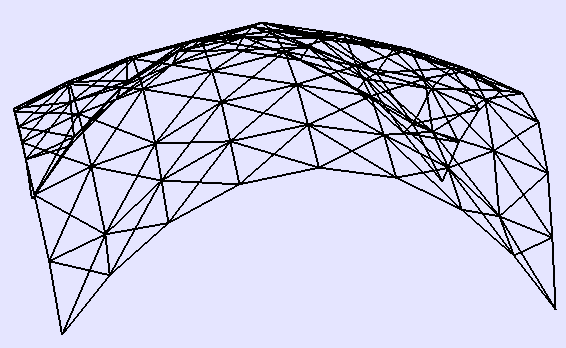
\includegraphics[width=3in]{images/simframe3.png}
}
\subfloat[]{
	\label{fig:wireframe_sim4}
	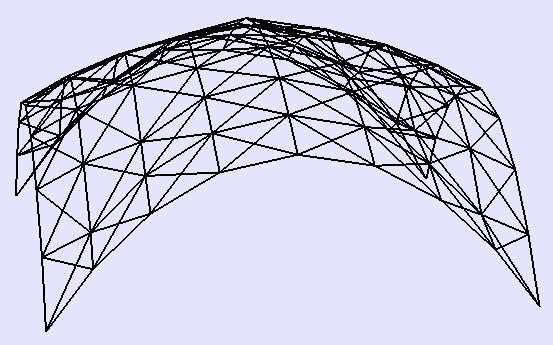
\includegraphics[width=3in]{images/simframe4.png}
}
\caption[Simulation frames]{These images show the motion of a shell as it is subjected to the simulation.  (a) is the starting position,
(b) shows the shell as the points begin to ``fall", (c) shows the shell as the points stop their free-fall, and (d) shows the equilibium
position.}
\label{fig:wireframe_sim}
\end{figure}

\begin{table}
\begin{center}
  \begin{tabular}{ | c | c | }
    \hline
    Number of points & Average FPS \\ \hline
	49 & 43.10 \\ \hline
	69 & 31.25 \\ \hline
    81 & 30.63 \\ \hline
	169 & 13.70 \\ \hline
    289 & 7.18 \\ \hline
  \end{tabular}
  \caption{Frames per second for various mesh sizes}
\end{center}
\end{table}

\section{Discussion}
There are numerous advantages to using an explicit midpoint integration method over other methods.  The midpoint method has a
considerable stability advantage over a first-order explicit integration, and is faster per frame than a fourth order Runge-Kutta
integration or implicit integration.  The stability increase over a first-order integration has the obvious benefit of being able to
take considerably larger time steps.  The spring correction allows for the imitation of very stiff springs without requiring very
small timesteps.  For a relatively small amount of clock time, the structure can be corrected in such a way that it remains stable
and avoids overstretching.

The primary disadvantage to an explicit solver rather than an implicit solver is that the timestep is limited.  However, while an
implicit solver can theoretically operate with arbitrarily large timesteps, the computation tradeoff is not favorable.  Furthermore,
the timestep used in the current simulation is large enough that the user does not grow impatient waiting for the structure to reach
equilibrium, nor is it short enough that the user cannot react to the motion of the shell.  An ancillary disadvantage to the
explicit solver is the necessity of correction methods to prevent overstretching.  However, this disadvantage is again offset by the
fact that even with the correction methods, the explicit solver is faster than an implicit solver.

\section{Summary}
The backend of this tool consists of a cloth data structure, to which a midpoint method solver is applied.  This solver is much more
robust than a first-order solver, but faster than an implicit solver or Runge-Kutta solver.  This speed makes it a great solution
for interactive tools such as this, and the robustness ensures that it is unlikely to become unstable.  On top of this solver is
added a correction method first suggest by Provot in \cite{provot95deformationconstraints} which reduces overstretching while
maintaining a large timestep.


\chapter{USER INTERFACE}
Now that a simulation engine had been created, a user interface could be created that would allow the user to interface with the
shell and create interesting shapes.  It was ver important for this interface to be both flexible and precise.  The user should
feel very in control over their structure, but also have the freedom to do make any shape they could come up with.  To allow this
control and flexibility, a multi-panel design was created, which can be seen in Figure \ref{fig:basic}.  The viewing window,
floorplan window, and grid window all work together to allow the user to create a wide variety of thin-shell structures.  Several
other UI elements are also available to the user which are not visible in the screenshot of Figure \ref{fig:basic}, but are
detailed in this chapter.

\begin{figure}
\resizebox{5in}{!}{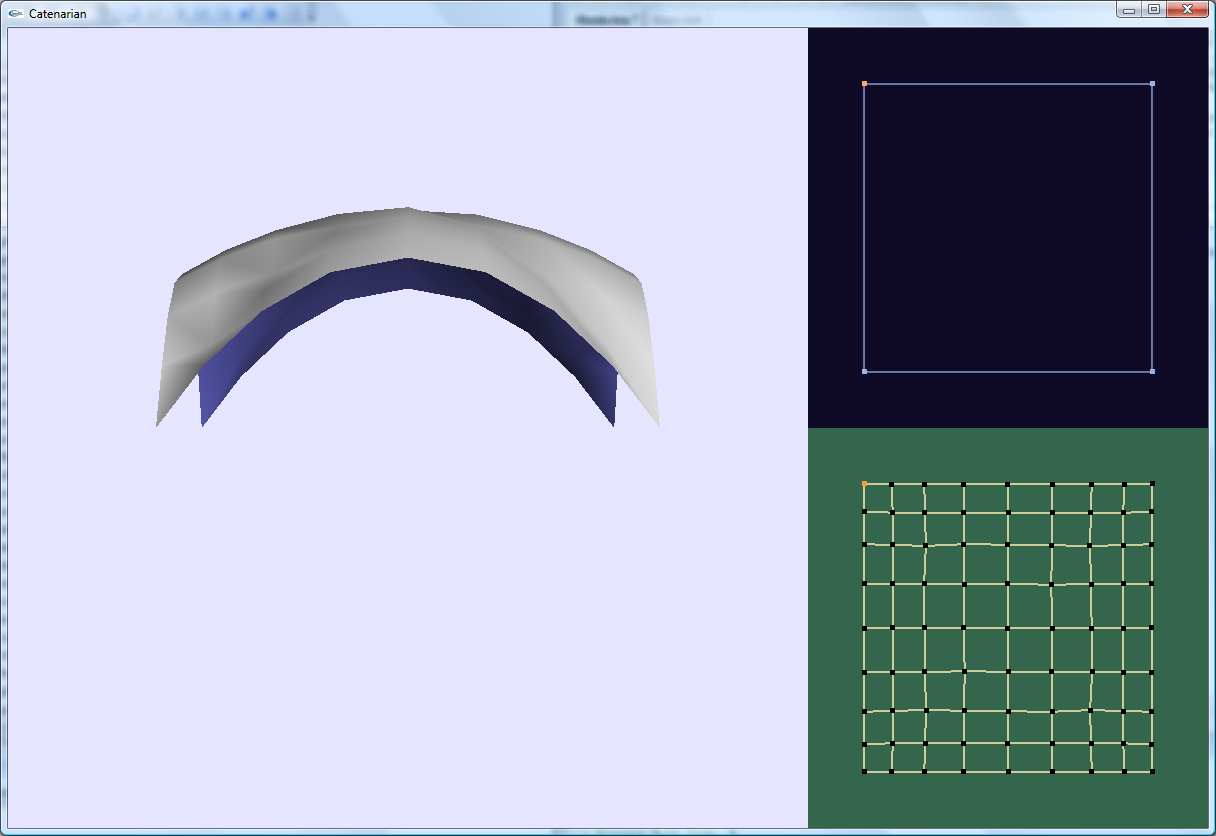
\includegraphics{images/basic.png}}
\caption[The tool]{This is a screenshot of the tool as it looks when first run.  On the upper-right is the floorplan window, and
in the lower-right is the grid window.  To the left is the viewing window with a view of the default shell.}
\label{fig:basic}
\end{figure}

\section{Vieiwing Window}
The first UI element that was created was a viewing window that allows the user to clearly view their structure as they make changes
to it. This window needed to have straightforward and expected camera controls: left-click and drag to rotate the camera, right-click and
drag to zoom, and middle-click and drag to pan the camera.  This window does not allow any control over the shell itself, only the viewing
of it.  The way to control the mesh would be through the floorplan and grid windows.

\section{Floorplan Window}
Since the item being designed is a thin shell, there will probably be a limited number of points touching the ground.  In order
for the structure to be stable, I decided that it made the most sense to manipulate these points and let the simulator take care
of placing the rest of them.  Since these points are all touching the ground, a floorplan view of these attached points seemed the
most sensible representation, as this would allow the user to manipulate the relevant points from a straightforward and uncluttered view.
However, simply being able to manipulate the points that exist when the shell is initially created is very limiting.  Therefore,
the creation of new points should be a central feature of the floorplan view.

The most intuitive method to add a new point is to simply click in the empty space in the floorplan view, so that is what was
implemented.  This makes it very easy to add new points to the floorplan.  Figure \ref{fig:waist} shows a shell with points that
have been added.  If the user wants to have a line of points attached to the ground rather than a single point in order to create
a wall or otherwise block off a portion of the shell, it can be tedious to add a point and place it correctly for every point along
the line.  Therefore, another feature in the floorplan view is the ability to attach a line between two points by right-clicking on
the line and selecting "Attach".  If they change their mind, a line can be freed by right-clicking on it and selecting "Detach".
Figure \ref{fig:barrel_vault} shows a simple shell with attached lines.  Lines can also be converted into a bezier curve to give
the user additional flexibility in designing their structure, as seen in Figures \ref{fig:thing_with_wings} and
\ref{fig:countercurve}.  Conversion from line to bezier is done by right-clicking on the line and selecting "Set Bezier".  To
convert back into a line, the user can right-click on the bezier curve and select "Set Line".

\begin{figure}
\resizebox{5in}{!}{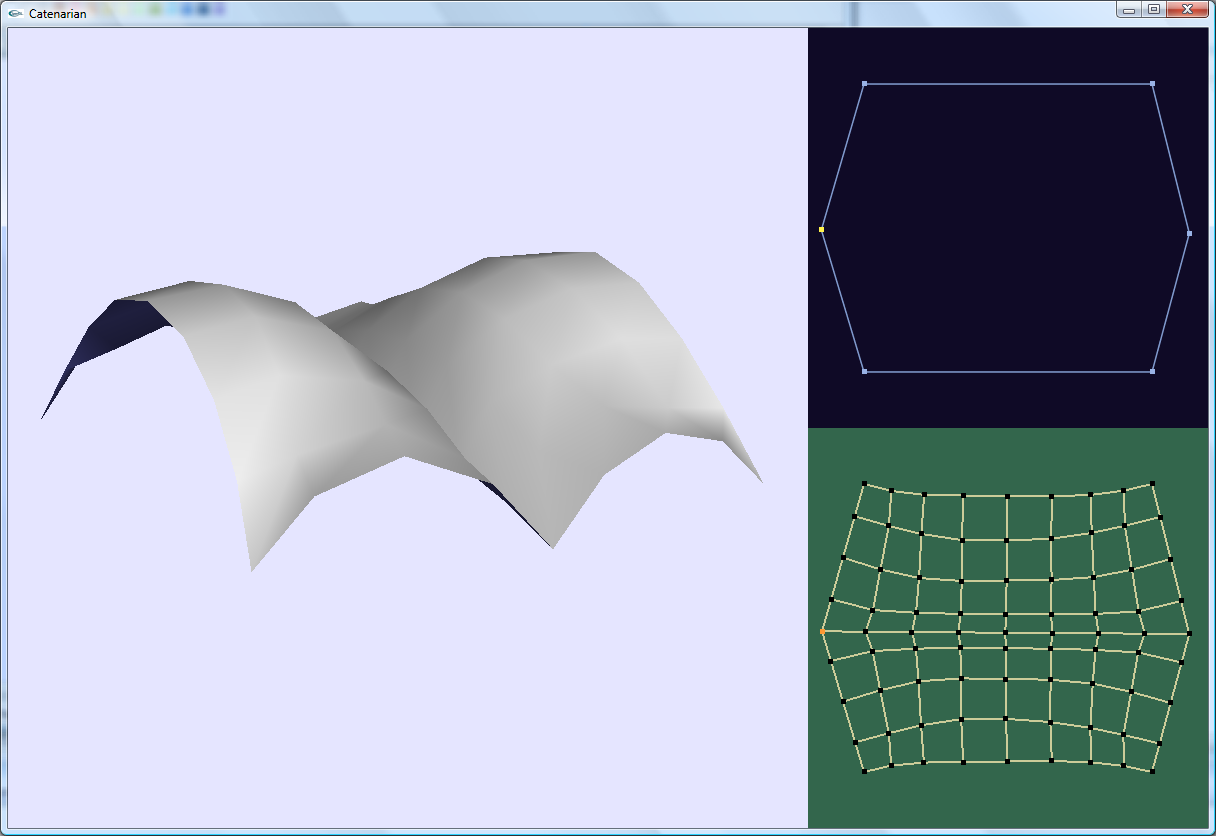
\includegraphics{images/waist.png}}
\caption[Adding points]{This shell was created by adding a point on either side of the square and attaching them.  This
caused the points in the mesh between the newly added points to be pulled down, forming a double-lobed shelter.}
\label{fig:waist}
\end{figure}

\begin{figure}
\resizebox{5in}{!}{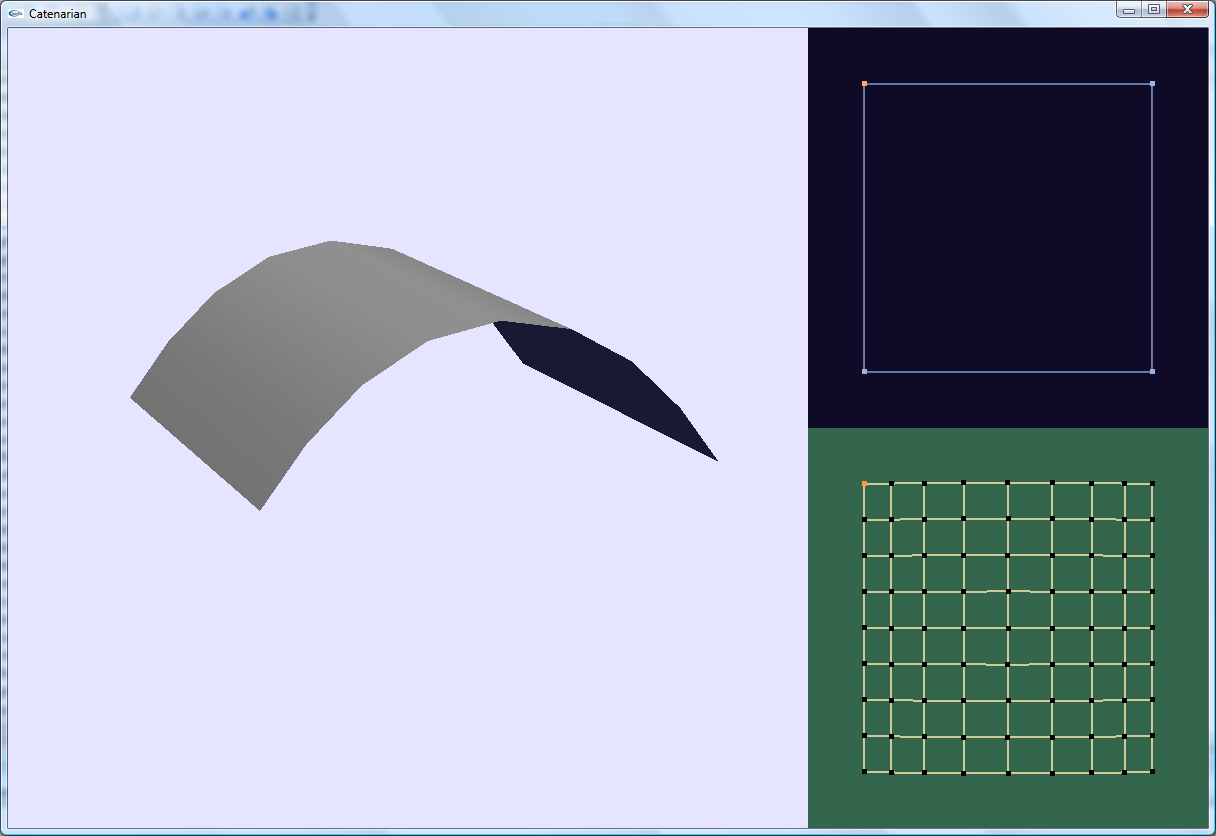
\includegraphics{images/barrel_vault.png}}
\caption[A barrel vault]{This barrel vault is created by attaching to parallel lines to the ground.}
\label{fig:barrel_vault}
\end{figure}

\begin{figure}
\resizebox{5in}{!}{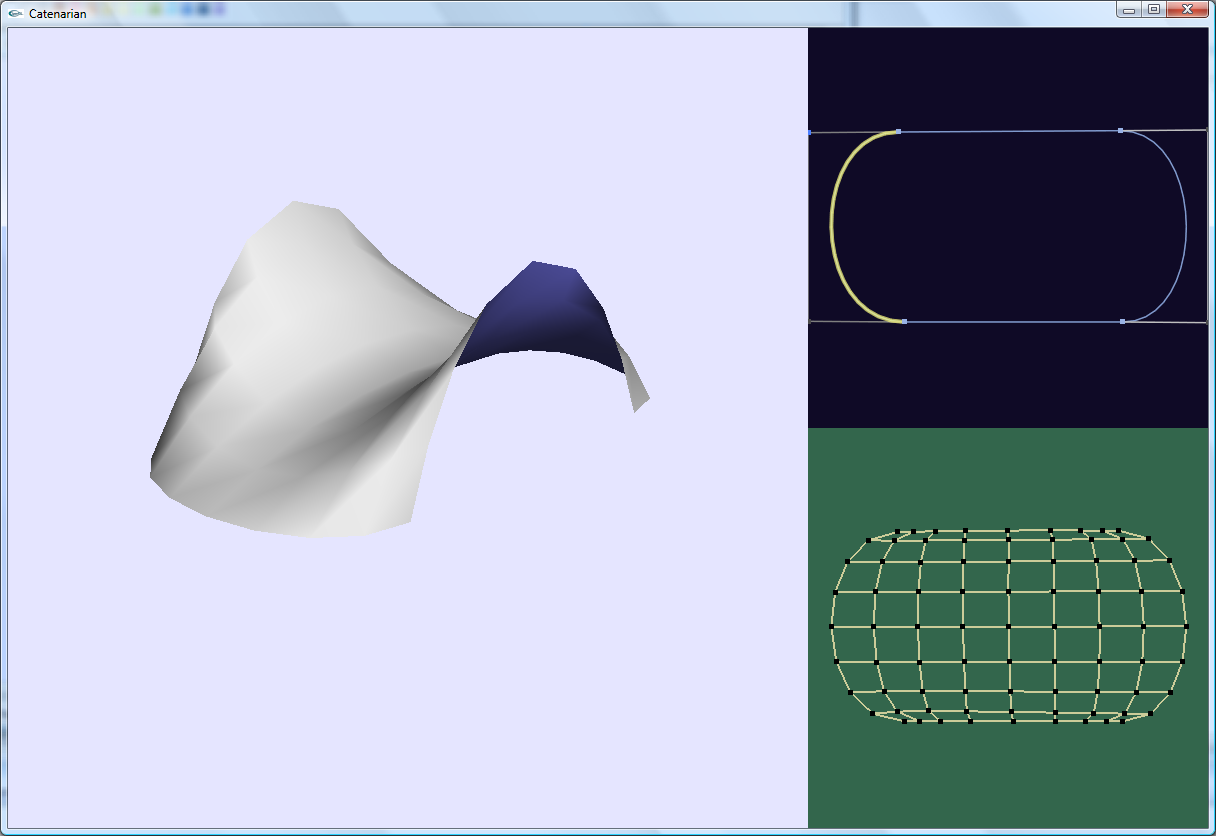
\includegraphics{images/thing_with_wings.png}}
\caption[Flared shell]{The flared edges on the sides of this shell are caused by the bezier curves on either side
allowing the edges of the shell to rise up.}
\label{fig:thing_with_wings}
\end{figure}

\begin{figure}
\resizebox{5in}{!}{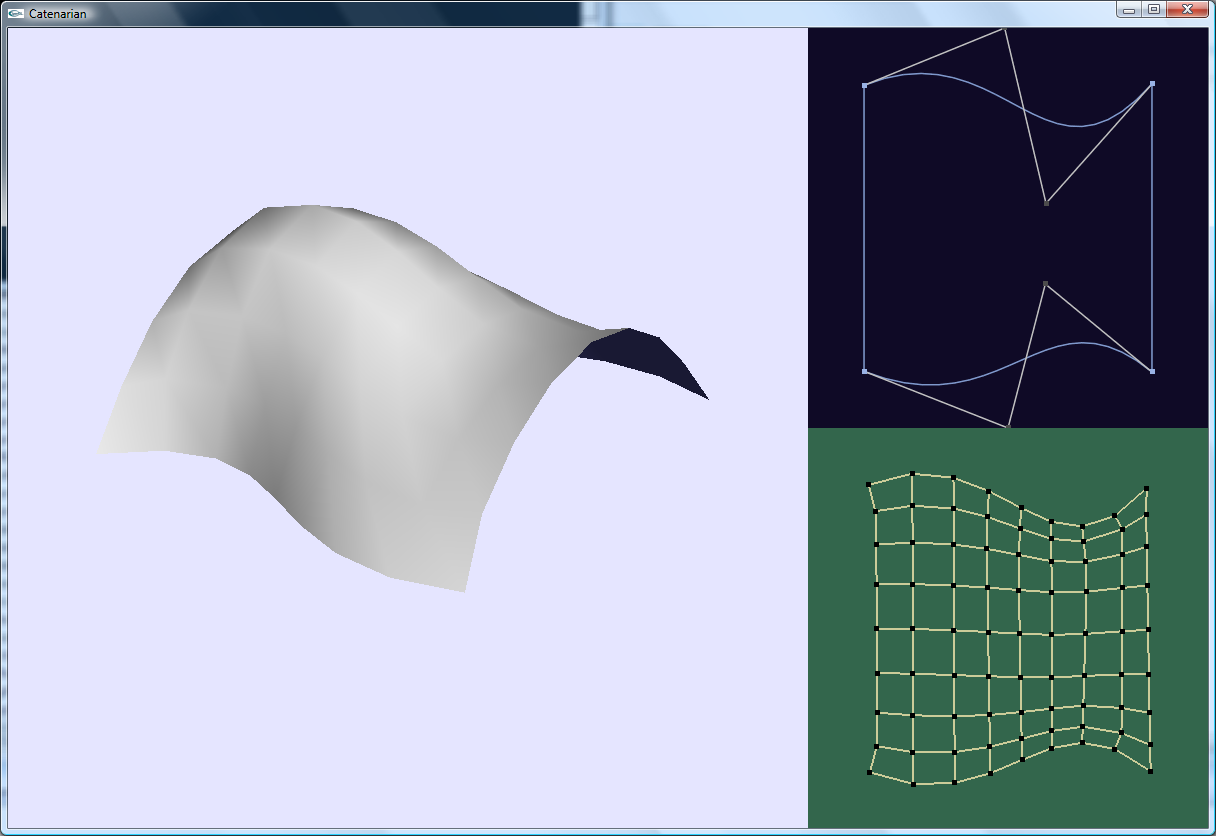
\includegraphics{images/countercurve.png}}
\caption[Modified barrel vault]{This shell, as well as the shell in Figure \ref{fig:thing_with_wings}, show some of the
interesting shapes that can arise from the simple barrel vault using bezier curves.}
\label{fig:countercurve}
\end{figure}

\section{Grid Window}
Once points are created in the floorplan, they need a context in the mesh in order to be meaningful.  Therefore, a window with
a two dimensional representation of the shell can be found in the lower right-hand corner of the window.  If a point is selected
in the floorplan, it can then be associated with a point in the mesh by clicking on that point in the grid window.  This causes
the point in the mesh that was clicked on to snap to the point on the ground corresponding to the selected point in the
floorplan view.  This mesh point can now be moved by dragging the associated point in the floorplan view.  One other
feature of the grid window is the ability to add windows or voids into the shell.  By right-clicking on a point, it is
removed from the simulation, thus creating a hole in the shell.  The shell in Figure \ref{fig:bird_windows} has a number
of windows in its sides.

\begin{figure}
\resizebox{5in}{!}{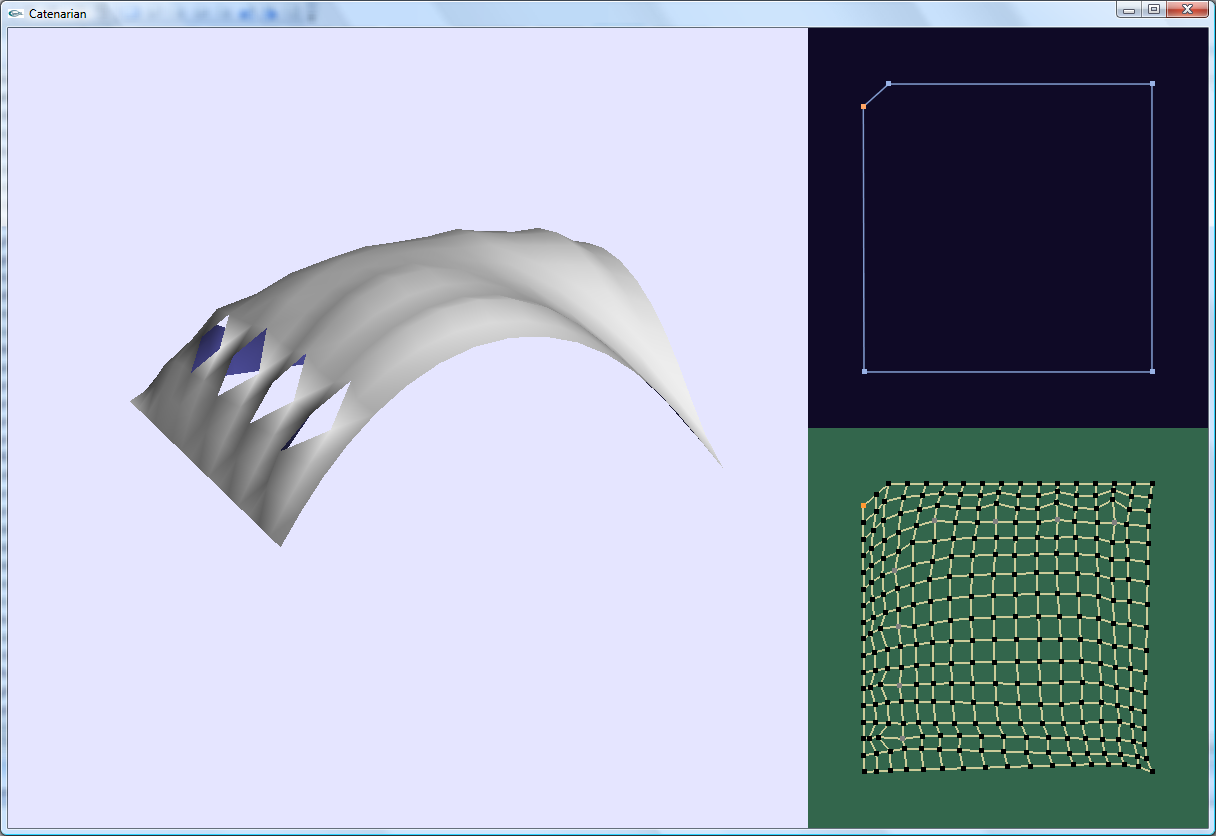
\includegraphics{images/bird_windows.png}}
\caption[Shell with windows]{This shell has one corner turned off and the points next to it attached to create the short wall
seen in the back of the space.  Also, points in the sides have been deactivated to create windows.}
\label{fig:bird_windows}
\end{figure}

\section{Other Features}
One problem that was discovered after the initial prototype had been created is that it can be very hard to select points if
there are a lot of them very close together.  To help combat this, the floorplan and grid windows zoom in when the user hovers
them, making the points more spaced out and easier to select.  Furthermore, the contents of each window was scaled so that the
points on the edges would be easier to select.  Figure \ref{fig:big_grid} shows the tool with the grid window enlarged.
Unfortunately, it is still possible for points to be directly above one another and therefore hard to select.  Alternate methods
of displaying the grid have been considered to help combat this problem.

\begin{figure}
\resizebox{5in}{!}{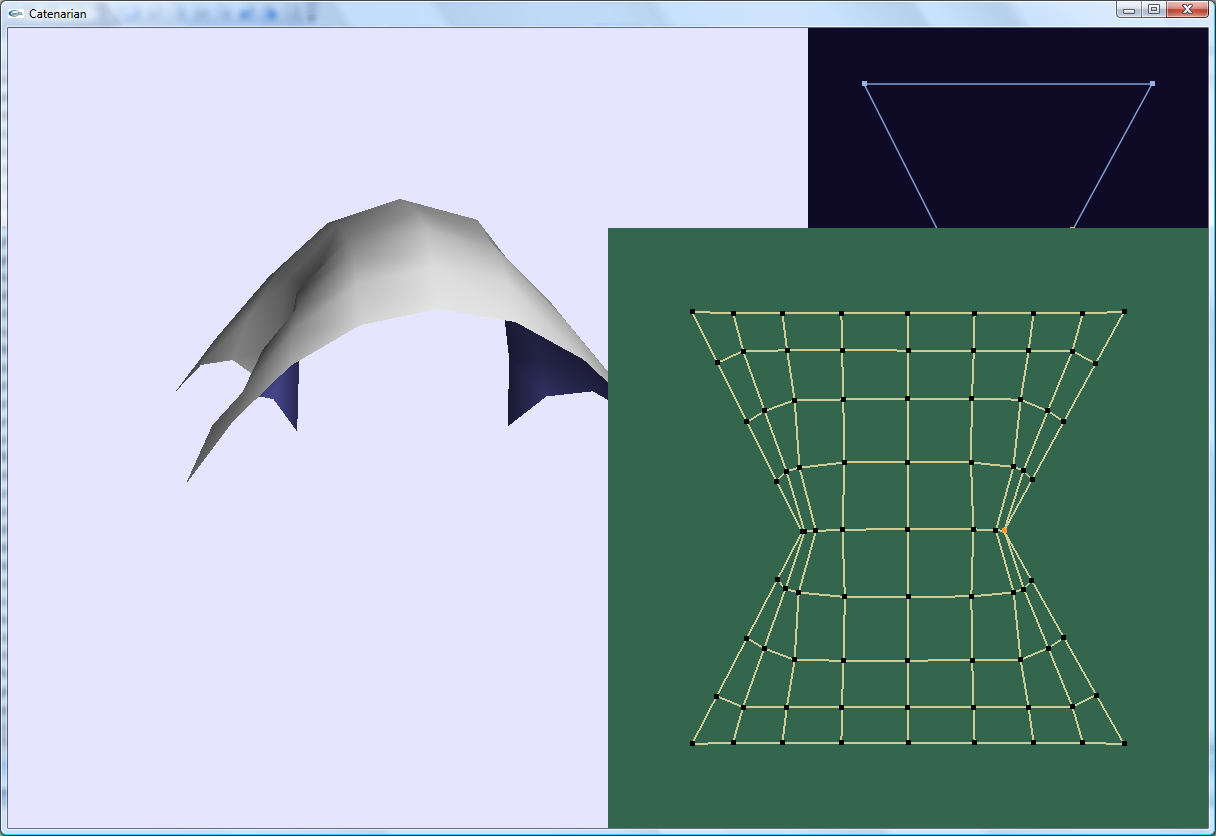
\includegraphics{images/big_grid.png}}
\caption[Zoomed in grid]{This screenshot shows the tool with the grid window enlarged.}
\label{fig:big_grid}
\end{figure}

One features that does not have an obvious UI elements associated with it is the ability to load shells that have been created
elsewhere.  If an architect has designed a shell in a traditional architectural CAD tool such as Rhino or Google SketchUp, they
can right-click in the floorplan window and select "Load input.obj" to load an exported mesh into the tool.  This allows users
to create a shell in an environment that they might be more comfortable in and import it into this tool so that the simulator
can adjust the mesh to be more structurally stable.  The shell in Figure \ref{fig:triangle_mesh} was loaded in this way.  No
restrictions are put on the shell to be imported, and the tool should be able to handle arbitrarily large or complex shells.
Additionally, if the user creates an interesting shell in the tool, they can right-click to save it.  The current implementation
of saving gives the file an automatically generated number to distinguish it from other saved files.  If the user would like to
start over from the initial shell, right-clicking in the floorplan window and selecting "Reset" will give the user a clean shell
from which to begin creating again.

\begin{figure}
\resizebox{5in}{!}{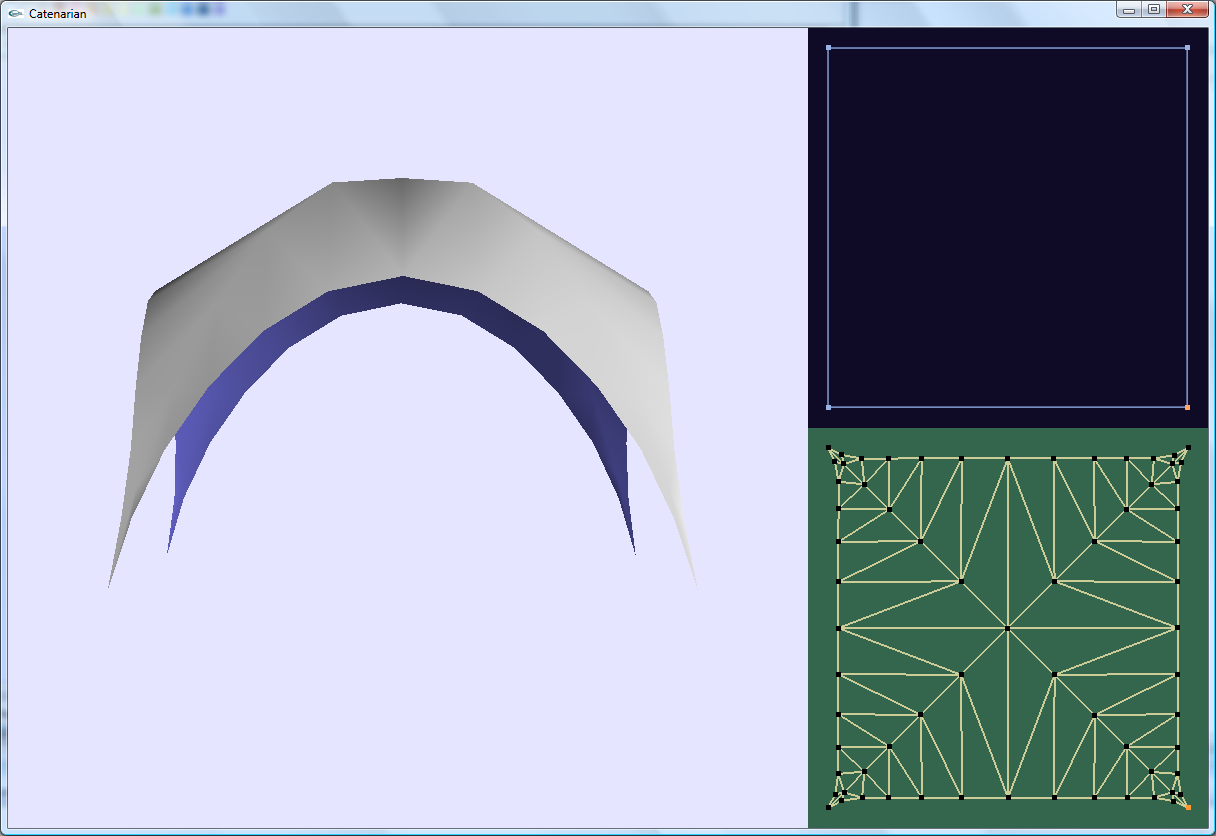
\includegraphics{images/triangle_mesh.png}}
\caption[A loaded mesh]{This shell was created in Google SketchUp, then imported into the tool, where it was optimized
from being semi-circular to catenary.}
\label{fig:triangle_mesh}
\end{figure}

One issue with the flexibility of the interface is that it allows the user to create impossible structures.  For example,
while the floorplan in Figure \ref{fig:highly_improbably} may look reasonable, when the connectivity of the shell is taken into
account it becomes apparent that the shell will be forced to intersect itself.  In Figure \ref{fig:inside_out_transient}, the
user has instructed the shell to turn inside out.  It will comply with this and be stable once it has finished simulating, but
its appearence as it goes to that state is a bit unusual.  Figure \ref{fig:tangle1} shows what happens when the user gives the
shell instructions that are completely impossible to follow.  While these structures would probably be buildable, I am not sure
whether or not they would in fact be stable.

\begin{figure}
\resizebox{5in}{!}{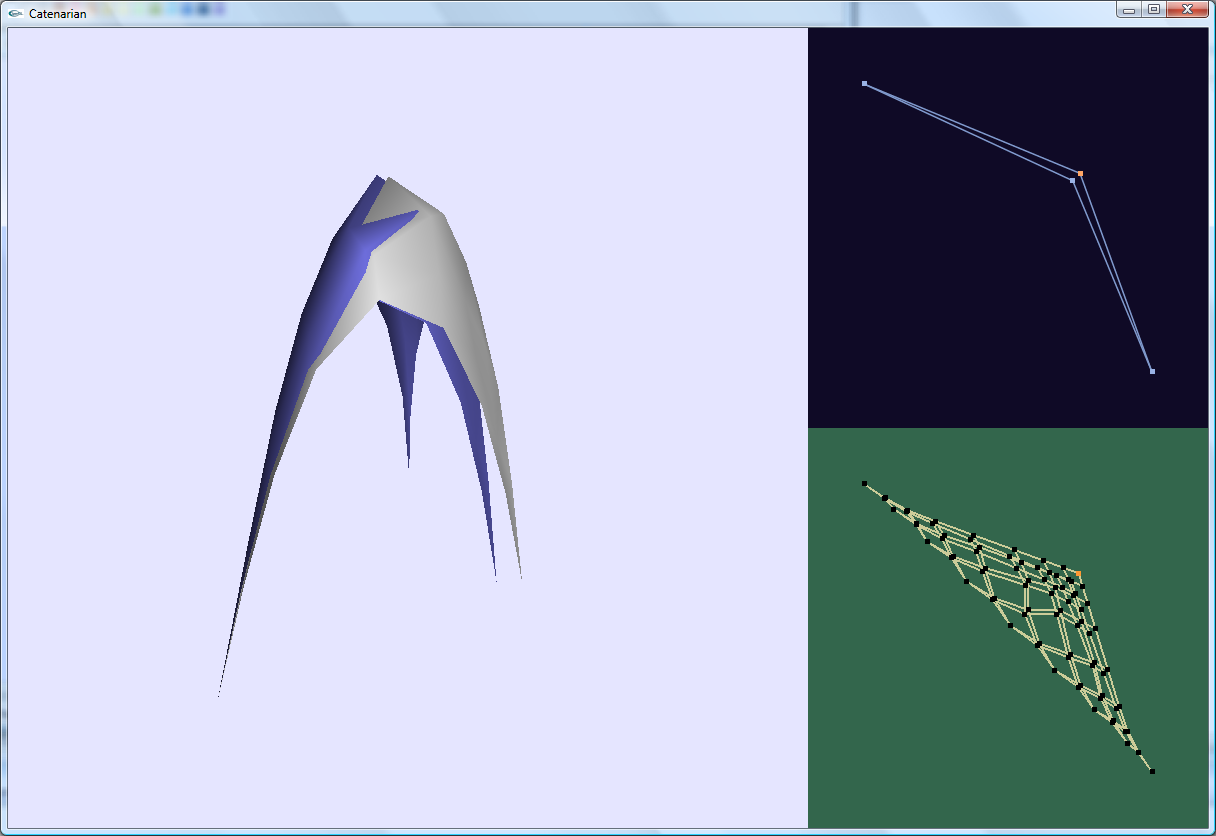
\includegraphics{images/highly_improbable.png}}
\caption[Results of user error]{While the tool tries to make every shape stable, there are some configurations of points
for which there no stable solution can be found.  For these, it finds the closest answer it can, which occasionally results
in the shell intersecting with itself.  In these cases, it is possible that the structure could be build, but the stability
is not guaranteed.}
\label{fig:highly_improbably}
\end{figure}

\begin{figure}
\resizebox{5in}{!}{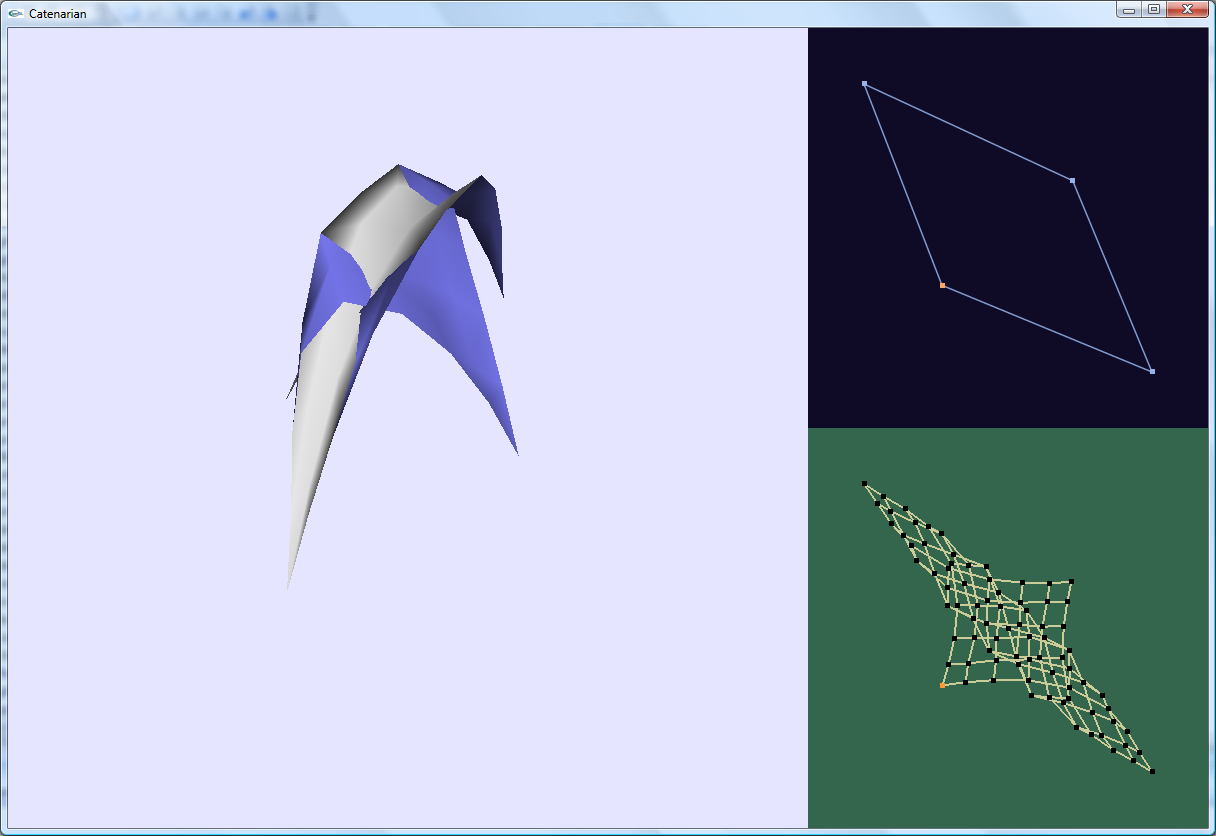
\includegraphics{images/inside_out_transient.png}}
\caption[Transient error]{This is a screenshot of a shell that is in the process of turning inside-out.  This screenshot does not
show an equilibrium configuration, and the inside-out equilibrium configuration will be stable, if unusual looking.}
\label{fig:inside_out_transient}
\end{figure}

\begin{figure}
\resizebox{5in}{!}{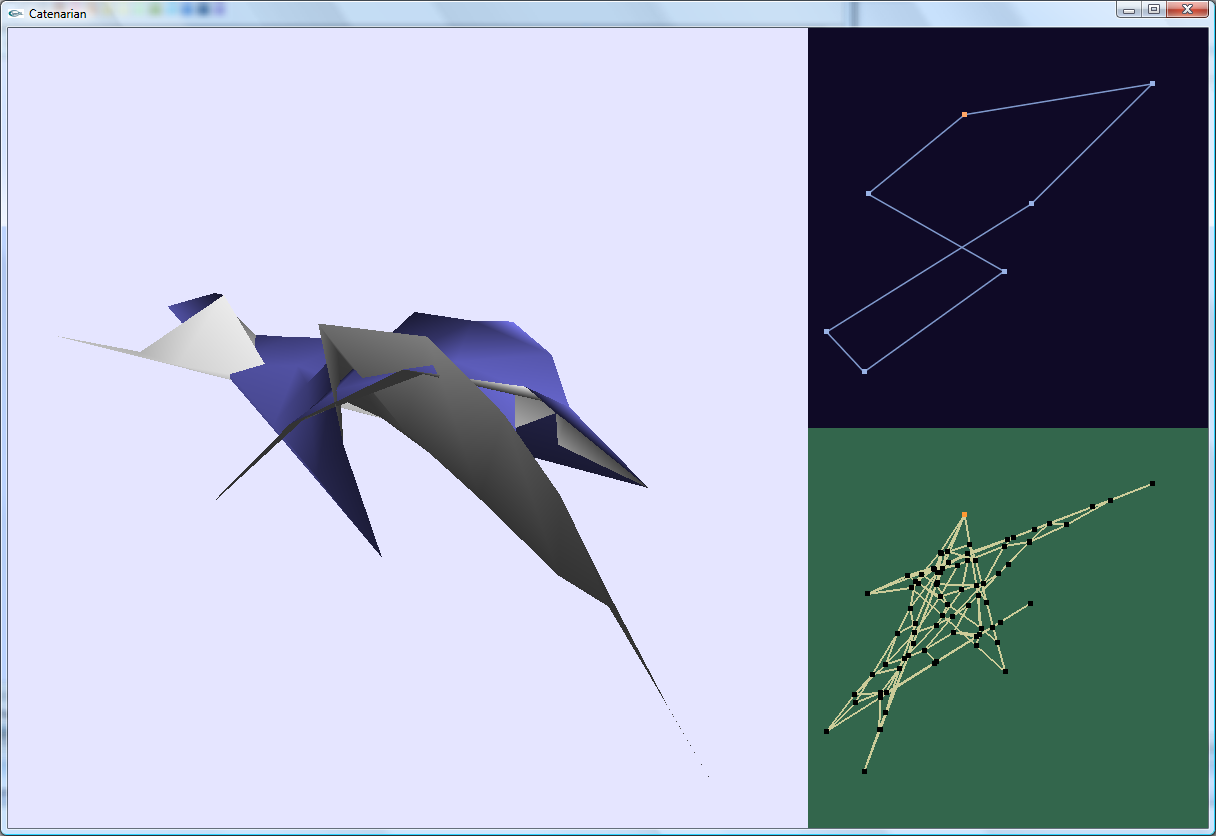
\includegraphics{images/tangle1.png}}
\caption[A tangled mess]{This screenshot shows what happens to a shell when the user pulls many control points through each other,
forcing the shell to contort strangely.  Shells such as this are unlikely to ever find an accurate solution, as the user has
instructed the shell to intersect itself in a number of places.  While this structure could probably be built, it would likely function
better as a sculpture than a structure.  The elegance of form and conservation of material that are the hallmarks of thin-shell
design are absent in designs such as this.}
\label{fig:tangle1}
\end{figure}

\section{Summary}
The user interface of this tool was designed with precision and flexibility in mind.  The viewing window has straightforward controls
to view a shell from any angle, while the floorplan and grid windows allow the user to make changes to the shell.  The floorplan
controls the fixed points and allows the user to attach lines and set them to bezier curves.  The grid allows the user to associate
floorplan points with points in the mesh and disable points to create windows.  Other tools available to the user are loading and
saving, resetting, and zooming the small windows.  Put together, these features make for a very flexible tool that allows users to
create a wide variety of thin-shell structures.


\chapter{USER STUDY}
Since this is a tool designed for users who do not share the same background as me, it was evident that a user study would have to be
conducted in order to get information on how useful the tool actually is.  In this section, I detail the process taken in designing
the study, then give observations taken as the users used the tool as well as responses given on questionnaires afterwards.  The user
study was the part of this project during which I learned the most about designing a useful piece of software, and I am taking several
lessons away from it.

\section{Design of the Study}
When designing the user study for this tool, the first consideration was what I wanted to get out of the study.  Being that this is
a design tool rather than a scientific tool, the results of a user study were liable to be rather subjective and not provide any hard
data.  Fortunately, subjective feedback is exactly what I wanted from this study.  My goal is for this tool to be useful and conform
to users' expectations while providing the functionality that they expect.  Therefore, the primary part of the study should involve the
user using the software, designing structures, and formulating an opinion of the tool.  Since very few software tools are immediately
intuitive, it was necessary for me to demonstrate the controls of the tool to the user before allowing them to use it.  While they used
the tool, I would watch, taking notes on their usage of the tool for use in improving the learning curve, bringing the controls
more in line with the expected functionality of existing architectural tools, and making other improvements to the software.  Any
comments they gave while using the tool were also noted, and ended up providing invaluable insights into the desired behavior of the
tool that were not reported anywhere else.  Once the user had used the tool for a sufficient length of time, they were directed to
complete a questionnaire which contained questions I had about their experience using the tool.

\section{The Questionnaire}
First and foremost on the questionnaire, I wanted to know what they liked about the tool.  Anything that stood out at them as
interesting or useful was something that I had succeeded in creating.  Secondly, I wanted to know which of a list
of potential features would be most appreciated by the users.  Users were asked to number various features with a 1-5, where
1 was ``not useful at all" and 5 was ``highly useful".  This would help me determine which feature was most important to
implement in the future.  Following this list, I asked users what other features they would like to see in the tool.  This
question resulted in a good list of ideas that had not previously crossed my mind.  Lastly in the basic tool questions, I
asked users to describe structures they could not make in the software that they felt it should be able to make.  This gave
me further ideas on how to improve the software by adding features that are capable of creating those types of structures.

In the next section of the questionnaire, I wanted to determine the usefulness of my tool in relation to existing tools.  Towards
this end, I asked the users to rate my tool versus existing tools in a variety of architectural applications.  This gave me a
better idea of how to market the tool to architects, as well as helping to direct my efforts in the development of the tool.
From this input, I was able to gain a more accurate picture of how architects saw my tool, compare that with what I
envisioned the tool to be, and formulate a plan to bring the two into closer alignment.

\section{The Users}
During the study, nine users were brought in to test the tool.  Four of them were architecture students, two were arts majors, two
were computer science students, and one was a civil engineering student.  Though the tool is aimed at architects, artists and civil
engineers can both use the tool in their work, and computer scientists can help detect other problems that may be present in the tool.
Each of the users spent about 45 minutes working with the tool and 15 completing the questionnaire.  All of the users came up with
different and interesting structures in their time with the tool.

\subsection{User 1}
\subsubsection{Interface Observations}
The first user I had in to use the software was an architecture student who was very excited about the software.
The first thing I noticed when he started using the software was that he tried to zoom with the mouse wheel.  That is a feature that
should be added.  Mouse wheel scrolling is a common functionality that should not be too hard to implement.

As he continued to use the software and get more comfortable with it, he noted that having left-click have an immediate action was not
what he was used to. Most architectural software allows the user to select points with the left mouse button, then right-click to
bring up the interaction menu.  Standardization would be a good idea.  This is especially true in the floorplan window, where
left-clicking places a new point, which is not what the user wants when they miss selecting a point by a few pixels.  On a related
note, an undo feature would be very welcome.  While it would be less of an issue if accidental left-clicks did not create points,
an undo feature would still help the user to revert changes, whether this reversion stems from error or indecision.

Something that became very clear to me as User 1 continued to use the software is that the current implementation of the mesh
interface is a bit clunky.  Firstly, when the user creates a new point in the floorplan view, the very next thing that is done is
usually to associate that point with a point in the mesh.  The mesh point chosen is usually the point in the mesh that is closest
to the location of the floorplan point, as shown in Figure \ref{fig:closest_point}.  To save the user a step, new points
should automatically associate with the closest point in the mesh upon creation.

\begin{figure}
\resizebox{4in}{!}{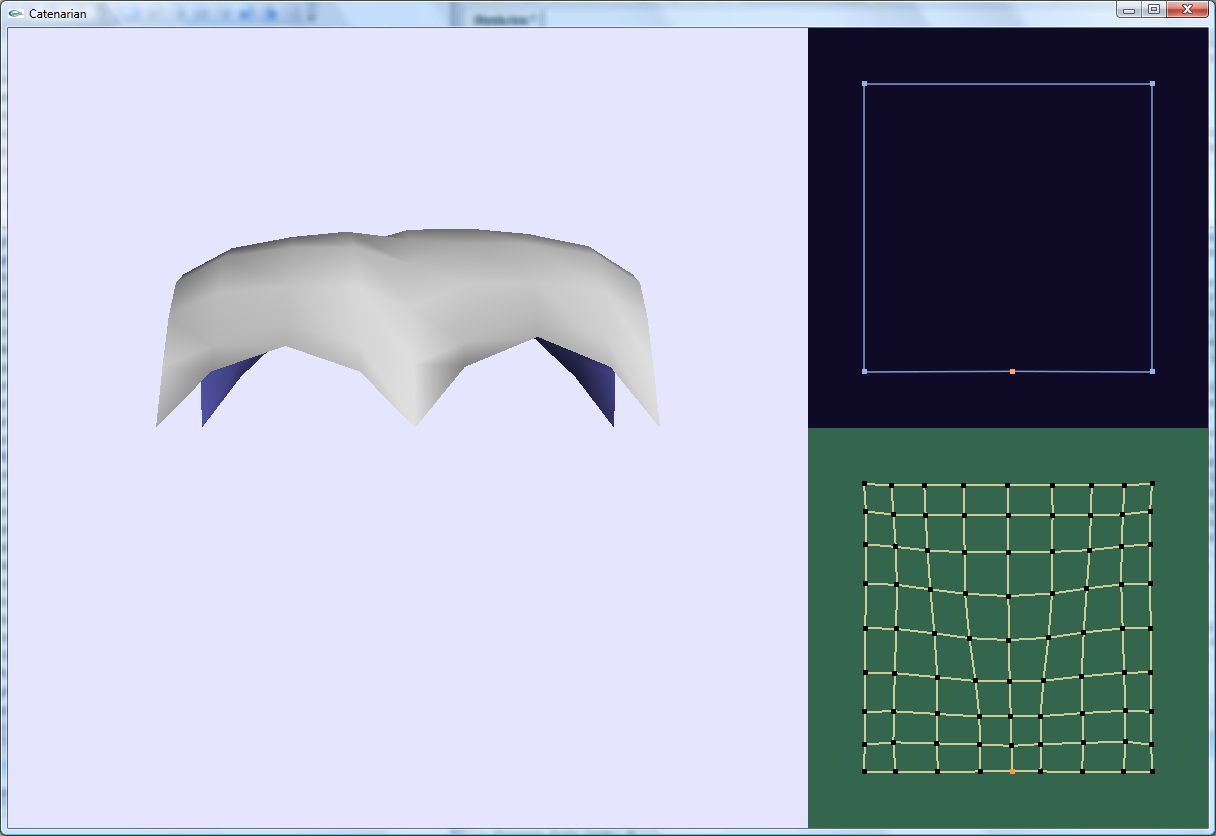
\includegraphics{images/closest_point.png}}
\caption[Association with the closest point]{This screenshot shows a shell after a point has been added in the floorplan and
associated with the closest point in the mesh.}
\label{fig:closest_point}
\end{figure}

Another problem with mesh association is the snapping of mesh points, shown in figure \ref{fig:snapping}.  Since the floorplan
point does not move when it is associated with a new mesh point, the mesh is forced to warp, sometimes drastically, to acquiesce
to the user's request.  The snapping is not a problem in and of itself; in fact it is the intended and expected behavior of the
tool.  The main problem with the snapping is that it surprises the user when it happens.  Having a less immediate interface would
help fix this.  Rather than left-click immediately associating the floorplan point with a mesh point, it should select the mesh
point, allowing the user to see which point on the mesh he was about to associate with a floorplan point.  He could then
associate the two via a right-click menu, which is a more natural workflow.  It also gives the architect finer control, allowing
them to have more information before making a change to the model.

\begin{figure}
\resizebox{4in}{!}{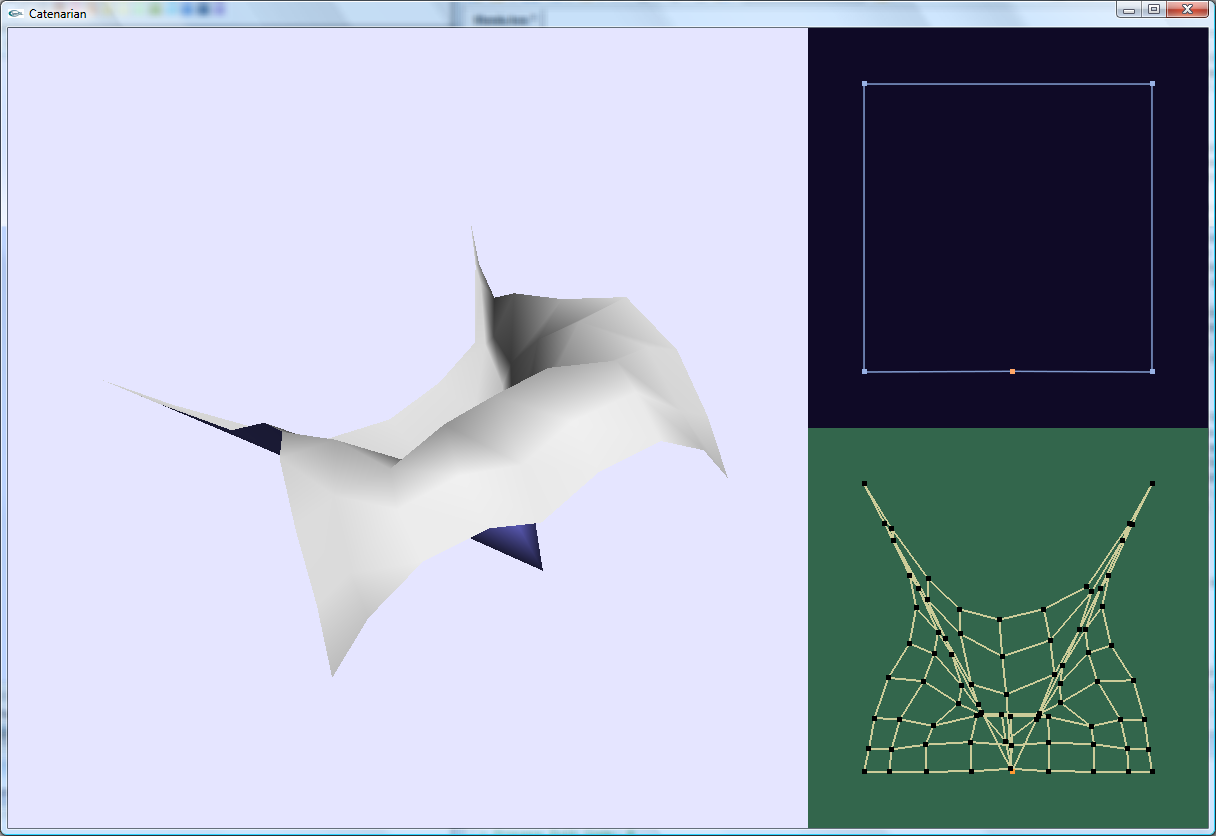
\includegraphics{images/snapping.png}}
\caption[Snapping]{This screenshot shows how the mesh is suddenly deformed when a mesh point is associated with a faraway
floorplan point.}
\label{fig:snapping}
\end{figure}

A workflow pattern that I noticed is that User 1 tended to start with an idea in mind of what he wanted to create.  Once that was made,
he would look at it from a few angles, then change it.  If the simulation started to get tangled up or if he made a mis-click
such that the model did something he was not expecting, he would continue to push it in that direction, ususally ending up in an
inescapable oscillation which would either require the mesh to be reset or crash the program.  I am not sure what was so intriguing
about the failures, but he seemed much more interested in them than in the successful structures.

\subsubsection{Feature Requests}
Some creative features that were requested include changing the height of points and length of springs.  Point height changing
would be a fairly simple feature, and allow for more complex catenary shapes that incorporate traditional structural parts.
Implementation would require adding a fixed height value to each point and adding a UI element to control this height.
Changing the length of springs would be a very useful feature, allowing the user to modify the shape of the structure in much
finer detail than is currently possible.  By manually tightening and relaxing springs, the structure can be allowed to slip into
any shape the architect wants.  This could be implemented by allowing springs in the mesh view to be clickable and having a UI
element to control their lengths.

Several visualization options were discussed during the trial, foremost of which was the option to highlight the selected floorplan
and/or grid point on the model.  This would make it much easier to orient the model to the floorplan and to keep one's bearings
when looking at the model from various angles.  Another visualization option that was requested was the ability to pause and rewind
the simulation of the model.  While rewinding is probably not feasible, pausing certainly is, though I am not certain that it is
necessarily a good idea since a model is not stable until it reaches equilibrium.

Several suggestions were also made with regards to audience and distribution.  User 1 suggested that this tool would work very well in
a web-based medium, perhaps with the ability for users to save and share their designs.  This could be a fun tool with potential for
collaboration.  In addition, it would be a great market to get a number of testers.  The downside to this, of course, is that this
would require a complete re-write of the code, as C++ is not well-supported on the internet.

\subsubsection{Questionnaire}
In his questionnaire, User 1 commented that he really liked the ``parametric design possibilities" that made it easy to ``quickly compose
catenary structures".  He thought that a variety of visualizations would be the most helpful features to add to the tool, especially
a visualization of materials and the ability to clearly see in the viewing window which points were selected.  One type of structure
that the tool cannot do easily that he was interested in making is ``structures with complex surface overlappings".

User 1 felt that this tool would be most useful in the design and meeting phases of construction, but less useful when preparing
designs to present to the client.  It best lends itself to inital concepts and optimization of design, but less to final design
development and presentation.

\subsection{User 2}
\subsubsection{Observations}
User 2 broke the tool considerably less often than User 1 had.  She tended to make interesting shapes that were well within the tool's
capabilities, using all the tool's features to make shells that were reasonable and useful.  It seemed that she was more interested in
simply using the tool than pushing it to its limit to find out exactly what it was capable of.

\subsubsection{Questionnaire}
User 2 thought that the way the floorplan and grid windows worked together was interesting and useful.  She felt it ``allowed for neat
designs to be created".  She also enjoyed the ability to create holes in the mesh.  User 2 felt that visualizations of material and
thickness would be the most useful features, with more robust saving and loading and the option to change the height of points being
a close second.  Like User 1, User 2 also felt that displaying the selected point in the viewing window would be very useful.  User 2
felt that this tool would be most useful during the conceptual design phase when creating a quick mock-up in 3D.  However, she felt
that it also has its uses at other points in the design process.

\subsection{User 3}
In his questionnaire, User 3 responded that he felt the tool provided an ``easy and intuitive way to quickly prototype and alter a
shell".  He also enjoyed it's support of bezier curves.  Unlike the previous two users, he felt that being able to save and load
shells more easily would be the most useful feature.  In addition, he requested a way to see which floorplan point was associated with
a given point in the mesh rather than only being able to see which mesh point was associated with a floorplan point.  In addition, he
requested the ability to change the lighting, as he found it hard to see the shell in some cases.

\subsection{User 4}
\subsubsection{Observations}
While using the tool, user 4 commented that it would be helpful to have a border around the floorplan and grid windows so that the
user was less likely to stray outside and inadvertently shrink the window.  The ability to disassociate floorplan points so that they
have no effect on the mesh was also requested, as well as an ability to snap lines in the floorplan view to angles.  He also felt
that it would be useful to be able to see all of the grid window when the floorplan window was enlarged and vice versa.  This would
require restructuring the layout of the interface, but could help the usability of the tool.  Also, the ability to move mesh points
within the grid window was requested.

\subsubsection{Questionnaire}
In his questionnaire, User 4 commented that he really liked the response of the shell when a point was moved.  A more sophisticated
saving and loading interface was selected as the most useful feature, while visualizations of materials and thickness rated lowest.
He felt that the ability to anchor points at heights other than ground level would be very helpful.  He also suggested that the ability
to associate with points in the viewing window rather than the grid window would be useful.

\subsection{User 5}
\subsubsection{Observations}
User 5 made some interesting shells, but kept running into a problem where the structure would oscillate due to an instability
somewhere in the structure.  She became very adept at quelling these oscillations, unlike User 1, who would try to find oscillations
then drive them into further oscillation.

\subsubsection{Questionnaire}
User 5 found the real-time visualization of the shell to be very useful.  She found the option to change the height of fixed points
to be the most useful potential feature, followed by the visualizations of materials and thickness.  She also wanted real-world
units to associate with the shells.  Even the addition of people to give a sense of scale would be useful to give the user some
idea of how big their structure was.  User 5 felt that there should be a way to have points going up as well as down when fixing
points.  She felt that this tool would be most useful in the design phase, as well as when presenting designs to the client.

\subsection{User 6}
\subsubsection{Observations}
User 6 felt that the camera controls in the viewing window were unintuitive.  She expected left-click to have an effect of the
structure and right-click to rotate the camera.  Also, the mouse wheel was expected to zoom.  She suggested the ability to
connect arbitrary points in the floorplan view so that it was easier to attach lines wherever the user wanted.  This would
require some restructuring of the floorplan structure, but would give the user a great deal of additional flexibility.

\subsubsection{Questionnaire}
In her questionnaire, User 6 stated that she found it ``very interesting to be able to watch the design shift as changes were made".
She also found the grid window to be an interesting way to represent that aspect of the structure.  She felt that all of the
suggested features would be useful, but found the visualizations of materials and thickness to be less useful than the others.
User 6 felt that the ability to tighten or loosen the shell would be very useful, as well as the ability to see a sense of scale.
One further suggestion was that the user be able to import a design from another tool, isolate that structure from the simulation,
and build a thin-shell structure on or in the imported design.  This user felt that this tool would be most useful during the early
design and final presentation phases of the project, but that it was less useful for team meetings.

\subsection{User 7}
In her questionnaire, User 7 stated that she felt that the ability to change the height of fixed points, as well as a more robust
saving and loading functionality would be most useful.  The other proposed features were considered less potentially useful.
User 7 felt that the thin-shell design tool would be most useful in team meetings and when presenting designs to clients rather than
in the schematic design phase.

\subsection{User 8}
In his questionnaire, User 8 stated that he thought this tool ``is a good program to design different shapes and interesting
structures".  He felt that the visualization of materials, a more robust saving and loading interface, and the ability to 
change the height of fixed points were the most useful suggested features.  He felt that the visualization of thickness was
particularly not useful.  User 8 felt the tool could be greatly improved by the ability to make multi-layer structures.
He felt the tool was most useful in the design phases, but that it was quite useful throughout the design process.

\subsection{User 9}
User 9 found the zooming of the floorplan and grid windows to be a bit disorienting, since the user can be aiming for a point
only to have it move as they approach the window.  In his questionnaire, he stated that once the user gets used to the tool,
it provides interesting methods of implementing designs.  He felt the learning curve was a bit steep, but had gotten used to
the tool well within his 45 minutes working with it.  As many of the other users had, User 9 felt that the option to change
the height of points was the most useful, with the visualization of the thickness being the least useful.  He felt that the
tool as a whole was most useful ``for ideation and conceptualizing thin shelled structures".


\section{Discussion}
\begin{table}
\begin{center}
  \begin{tabular}{ | p{3in} | c | }
    \hline
    Feature & Average usefulness \\ \hline
	save/open dialog & 3.78 \\ \hline
	option to change the height of points & 4.22 \\ \hline
	visualization of the difference between an imported mesh and the optimized mesh & 3.44 \\ \hline
	visualization of materials used in the structure & 3.56 \\ \hline
    visualization of the thickness of the structure & 3.22 \\ \hline
  \end{tabular}
  \caption{Average usefulness of various features}
  \label{tbl:features}
\end{center}
\end{table}
	%1 4 5 4 2 5 5 5 3 = 3.78
	%2 4 4 3 5 5 5 5 5 = 4.22
	%3 3 3 3 3 5 3 4 4 = 3.44
	%5 5 3 2 4 3 3 5 2 = 3.56
	%4 5 3 2 4 4 4 2 1 = 3.22

Table \ref{tbl:features} shows the usefulness of various features, rated on a scale from 1 to 5.  These values are averaged from
the responses of the 9 users.  Unfortunately, many of the users had very different ideas of what as important, so most of these
averages do not mean much.  I can conclude that the option to change the height of fixed points is the most valuable feature,
since is has not only the highest average, but also the highest median and mode, both of which are 5.  The visualization of the
difference between an imported mesh and the optimized mesh sits solidly at "average", with 6 users rating it a 3.  However, the
other three features had a wide and even distribution of ratings, so no solid conclusions can be drawn from the data.  One
possible cause for this variation is that several users were confused by the instruction to rate these features from 1 to 5,
thinking that each number could only be used once.  This caused some features to be rated lower than the user perhaps intended
them to be rated, which causes undue variance in the data and makes the averages rather meaningless.

The responses when asked to rate the usefulness of the tool in various situations showed even more variance than the previous
question, and is therefore not statistically significant.  However, from the users' written responses, it was mostly agreed
that the tool is most useful in the design stages of a project and less useful in meetings.  Overall, the users found the tool
to be interesting and useful, offering flexibility and possibilities for design.  While some users found issues with the tool,
they all created interesting structures and had good suggestions on how to improve it.

One large realization I had while performing this user study is that I should have had other people look at the tool while it
was still in its early stages.  While I have been and still am a fan of iterative design, I neglected to consult other people's
input until very late in the project.  While I knew exactly how my tool worked, what I wanted out of it, and all its little
idiosyncrasies, I did not allow other people to use my software until it was in a ``stable" state.  Once I conducted my user study,
a number of issues were brought to my attention, some of which would have been very easy to fix, add, or modify if I had known
about them earlier in the life cycle of the tool.  Many of them are still easy to deal with, but more smaller user studies
would probably have been more useful than the one larger user study.

\section{Summary}
In this chapter, I discussed the user study that was conducted as a part of this project.  Observations, suggestions, and
questionnaire responses from the 9 users are detailed in this chapter, followed by a discussion of the overall results of the study.
As a whole, the users found the tool to be quite useful and provided a number of great ideas on how to improve it to be even more
useful.


\chapter{FUTURE WORK}

\section{Changes to existing features}

\subsection{Cloth}
When I originally wrote the cloth simulation code for this project, I was under the impression that implicit integration methods were
too slow for use in an interactive project.  However, I recently happened upon the paper ``Comparing efficiency of integration methods
for cloth simulation"\cite{volino01comparingefficiency}\nocite{volino00fastcloth}, which reports that a properly implemented implicit
solver is as fast as, if not faster than, a midpoint explicit solver.  In addition to being nearly as fast per timestep, the implicit
solver is also stable for considerably larger timesteps than can be comfortably used with the explicit solver.  With this new
information in mind, I would very much like to replace the current cloth simulation with an implicit method, as that will eliminate
several of the issues I find fault with in the program.

\subsection{Clicking}
In the current implementation, left-clicking in the floorplan pane places a new point and left-clicking in the grid pane associates
the currently selected point with the point that was clicked on.  Both of these behaviors are unexpected to many architects.
Traditionally, architectural software has the pattern that left-clicking is only for selection and right-clicking is used to interact
with selected objects.  Therefore, an interface change to improve the learning curve will be to alter the grid pane such that
left-clicking selects a point and right-clicking brings up a menu with the options to associate/deassociate and disable/enable that
point.  In the floorplan pane, left-clicking in empty space will deselect all points, and to create a new point the user must
right-click and select the ``new point" option from the pop-up menu.

A related issue is that the precision required to select points in both the floorplan and grid windows is a bit high.  Increasing
the radius from which points can be selected will help the usability of the program, as it will result in fewer mis-clicks.

The viewing window also has an unusual button layout.  Architects seemed to expect right-click and drag to rotate, while the mouse
wheel was expected to zoom and middle click was not really used at all.  Panning would then be delegated to left-click.

\subsection{Floorplan}
Points start free, can be associated at will FINISH THIS

\subsection{Save/Open option}
There is a save option and an open option, but neither of them is really what it should be.  The save option saves automatically
numbered files into an automatically generated folder, while the load option loads a hardcoded filename.  Both of these options
should have a dialog box of some sort to allow the user some control over what is saved and loaded.

\subsection{Other}
I know there are other things I wanted to change; I'll fill this in later.

\section{Additional features}

\subsection{Height change}
One feature that was commonly requested was the option to change the height of a fixed point.  This would allow structures built
in this tool to more easily interface with existing structures, as well as giving architects further control over the final form
of the structure.

\subsection{Visualizations}
There are a few visualization options that would be very nice to have in this tool.  One which is not as useful at the moment due
to the awkward loading interface is the ability to visualize the difference between the loaded structure and the structure after
optimization.  This would aid the architect using the software in determining which parts of the structure that was imported
changed the most.  In many cases, the shift from imported mesh to optimized mesh is very slight, being the difference between
a hemisphere or parabola and a catenary.

Another visualization which comes with a change to the simulation is a visualization of the thickness of the structure.  Parts
of a shell which have higher loads must be thicker than the parts with smaller loads in order to support the load.  For example,
in Figure \ref{fig:isler_service}, the corners of the dome are much thicker than the center of the roof because they must support
a great deal more weight.  The simulation does not currently differentiate between thin and thick portions of the mesh, so that
attribute would need to be added before this visualization could be implemented.

One other visualization that could be added is a visualization of material.  The ability for a user to customize the material the
structure is made of has a huge effect on the aesthetic of the structure.  Possible presets could include concrete, which would be
rather similar to the current material; glass, which would require rendering of the lines and specularity on the faces, and wood,
which would require a texture to be applied.  For further flexibility, the user could have direct control over the colors, textures,
and material properties of the materials present in their structures.

\subsection{Other}
There are other features; I need to remember what they are (i.e. read questionnaires again)

\section{Other possibilities}

\subsection{Grasshopper}
One possible future for this project is as a plugin for the architectural CAD software Rhino.  Since architects have a
somewhat cumbersome workflow as it is, adding an additional tool that requires importing and exporting their design is
perhaps more than should be expected of them.  Towards this end, creating a plugin for software that is the primary part
of their normal workflow would make the software much more accessible and useful.  Grasshopper is a tool that allows procedural
creation of features within Rhino.  If a plugin were made in Grasshopper, architects could create a shell in the software that
they would use to create it anyway, run a script on the model, and get the benefits of this software with the press of a
button.  One major roadblock to this deployment method is that in order to create a Grasshopper plugin, the software would
need to be rewritten from scratch.  While the algorithms and UI design could probably be kept the same, a complete rewrite
is still a major undertaking.

\subsection{Web application}
Another potential distribution method for this software is as a web application.  The advantage to the web platform is that the
user does not have to download anything, which makes it much more likely that an architect would try it out.  Furthermore, the
web is a great environment for collaboration.  With a properly designed app and website, a collaborative thin-shell structure
community could be created where architects and artists can create structures, share them, comment, and collaborate in the
design of interesting, stable structures.



\chapter{CONCLUSIONS}
Overall, this project was a success.  I created a tool that architects enjoyed using and learned a lot about architecture and
software development in the process.

Before starting on this project, I had a basic knowledge of architecture and statics, as well as a rudimentary definition of what
a thin-shell structure is.  I had taken an architectural CAD class in high school, and have experience in both wood and cinderblock
construction.  However, while the basic architecture knowledge was useful, none of it was particularly relevant in the wild world
of thin shells.  Thin-shell structures tend to break all the traditional ``rules" of construction, supporting themselves through
thin, flowing elements rather than the straight, rigid structural elements that are the hallmark of traditional construction.

In my first attempt at a thin-shell design tool, I used Ruby to create a plugin for Google SketchUp that would attempt to analyze
a structure created in SketchUp and indicate which elements of the shell were under tension and which were under compression.
However, the solution method I used in this plugin did not behave very well on most shells.  This is because the method I was
using to solve the system of equations is not very well suited to sparse matrices.  I have since learned of more appropriate
solving methods, but the method I used is what I was familiar with at the time.  After determining that the plugin was not
very effective as it was, I decided to abandon the idea of a SketchUp plugin, as the Ruby interface was not as powerful as I had
hoped it would be, nor was it fast enough to deliver the interactive experience I wanted from it.  Therefore, this design was
scrapped in favor of a standalone c++ tool.

The development of this tool was the most valuable development experience I have had, as it gave me practical insight into some
parts of software development I had never experienced before.  

Secondly, I gained a great deal of practice using OpenGL and c++, as well as various tools.  Since I was designing this tool for
Windows in order to have the largest potential market audience, the use of Visual Studio was recommended.  Since most of my
previous c++ experience had been in Linux or Cygwin, it was quite a pleasant surprise to get to know all the powerful features
that Visual Studio had to offer.  Another tool that proved invaluable in the creation of this tool is Very Sleepy, a performance
profiler.  The ability to see what exactly a program is doing is very useful when trying to determine what is causing said
program to slow down.

While I had used OpenGL before, I had never dealt with multiple windows before.  This was an interesting challenge, since all
three windows needed to be able to render the others at various times throughout the execution of the program.  This problem,
along with the performance optimization required to make the simulation interactive and the challenge of creating a user
interface from scratch taught me many practical lessons about c++ that will doubtlessly be useful on future projects.


% The following produces a numbered bibliography where the numbers
% correspond to the \cite commands in the text.
\specialhead{LITERATURE CITED}
\begin{singlespace}
\bibliographystyle{unsrt}
\bibliography{thesis}
\end{singlespace}

%%%%%%%%%%%%%%%%%%%%%%%  For Appendices  %%%%%%%%%%%%%%%%%%%
\appendix    % This command is used only once!
\addtocontents{toc}{\parindent0pt\vskip12pt APPENDICES} %toc entry, no page #
\chapter{QUESTIONNAIRE}
\setlength{\parindent}{0in} 
{\bf PART 1: THIN SHELL TOOL} 
\hfill Participant ID \verb+_______+
\vspace{0.3in}

What did you think was useful or interesting about this tool?
\vspace{1.1in}

Please rate the following potential features from 1-5, where 1 is not useful at all and 5 is highly useful: \\

\verb+___+ save/open dialog\\
\verb+___+ option to change the height of points\\
\verb+___+ visualization of the difference between an imported mesh and the optimized mesh\\
\verb+___+ visualization of materials used in the structure\\
\verb+___+ visualization of thickness of the structure


\vspace{0.3in}

Please list any other features that would have been useful in designing thin-shell structures.
\vspace{1.2in}




Describe or sketch some structures that you were unable to create due to limitations of the software.
\vspace{1in}



\newpage
{\bf PART 2: DESIGN METHOD COMPARISON} 
\hfill Participant ID \verb+_______+
\vspace{0.3in}

Rate the usefulness of various design tools in the following scenarios from 1-5,
where 1 is not useful at all and 5 is highly useful:


Schematic Design (early-stage architectural design)\\
\verb+___+ paper \& pencil sketching \\
\verb+___+ traditional computer software \\
\verb+___+ thin-shell design tool \\
Team design meetings with architects \& engineering consultants\\
\verb+___+ paper \& pencil sketching \\
\verb+___+ traditional computer software \\
\verb+___+ thin-shell design tool \\
Presentation of preliminary or final designs to the client\\
\verb+___+ paper \& pencil sketching \\
\verb+___+ traditional computer software \\
\verb+___+ thin-shell design tool \\


Additional comments or scenarios where these methods are most useful
\vspace{0.15in}

\hspace*{0.3in} 
Paper \& pencil sketching:
\vspace{0.7in}

\hspace*{0.3in} 
Traditional computer software:
\vspace{0.7in}

\hspace*{0.3in} 
Thin-shell design tool:
\vspace{0.7in}

Are there any other design tools that would be more useful than those listed above
in any of the scenarios?


\newpage
{\bf PARTICIPANT BACKGROUND \& EXPERIENCE}
\hfill Participant ID \verb+_______+
\vspace{0.3in}

\renewcommand\arraystretch{2}

\begin{tabular}{l@{\hspace{0.3in}}l}
Completed degree(s): 
& \verb+______________________________________+ \\
Degree(s) in progress: 
& \verb+______________________________________+ \\
%
\begin{minipage}[b]{1.8in}
\begin{flushleft}
~\\~\\\# of years of \\ architectural \\ education:
\end{flushleft}
\end{minipage}
& \verb+______________________________________+ \\
%
\begin{minipage}[b]{1.8in}
\begin{flushleft}
~\\~\\\# of years of \\ visual arts education:
\end{flushleft}
\end{minipage}
& \verb+______________________________________+ \\
%
\begin{minipage}[b]{1.8in}
\begin{flushleft}
~\\~\\\# of years of \\ architectural experience \\ (internships/jobs): 
\end{flushleft}
\end{minipage}
& \verb+______________________________________+ \\
%
\begin{minipage}[b]{1.8in}
\begin{flushleft}
~\\~\\\# of years of \\ visual arts experience \\ (internships/jobs): 
\end{flushleft}
\end{minipage}
& \verb+______________________________________+ \\
%
\begin{minipage}[b]{1.8in}
\begin{flushleft}
~\\~\\other relevant education/experience \\ (please describe):
\end{flushleft}
\end{minipage}
& \verb+______________________________________+ \\
%
\end{tabular}

\renewcommand\arraystretch{1.0}

\vspace{0.5in}

\newpage
{\bf CONSENT FOR PUBLICATION}
\vspace{0.1in}

After completing this survey:
\vspace{0.3in}

\verb+____+~~
\begin{minipage}[t]{5.8in}
I give permission for use of any or all of the thin-shell designs
and my comments in academic
publications. This information will be anonymous and my participation
in the study will not be revealed.
\end{minipage}
\vspace{0.3in}

\verb+____+~~
I give permission for use of selected information.  (please describe)
\vspace{0.3in}

\verb+____+~~
I do not give permission for use of any of this information at this time.


\newpage
{\bf PARTICIPANT CONTACT INFORMATION}
\hfill Participant ID \verb+_______+
\vspace{0.3in}


RPI requires us to collect the following basic contact information
from all participants in this user study.  Your participation will
remain confidential, and this portion of the record will be securely
stored by Professor Barbara Cutler.

\vspace{0.2in}

\renewcommand\arraystretch{2.0}

\begin{tabular}{r@{\hspace{0.3in}}l}
Name: 
& \verb+______________________________________+ \\
E-mail: 
& \verb+______________________________________+ \\
Home mailing address: 
& \verb+______________________________________+ \\
& \verb+______________________________________+ \\
& \verb+______________________________________+ \\
\end{tabular}

\renewcommand\arraystretch{1.0}

\vspace{0.5in}

Participants for this study will be compensated for their time in the
form of a gift certificate at the rate of \$10 per hour.  This
compensation is not contingent upon the subject completing the entire
study and will be prorated if the subject withdraws.  For IRS income
reporting purposes, RPI must also collect the social security number
and RIN number of participants who accept compensation. 
\vspace{0.1in}

\renewcommand\arraystretch{1.75}
\begin{tabular}{r@{\hspace{0.3in}}l}
\hspace{0.45in}Social Security number:
& \verb+______________________________________+ \\
\hspace{0.45in}RIN number:
& \verb+______________________________________+ \\
\verb+______+ & I decline the compensation
\end{tabular}

\renewcommand\arraystretch{1.0}

\newpage

\vspace*{0.5in}

Thanks for participating in our user study!\\

\vspace{0.2in}

Allan Pendergrast\\
Masters Student\\
Department of Computer Science\\
Rensselaer Polytechnic Institute\\
{\tt pender@rpi.edu}\\
\url{http://www.rpi.edu/~pender/}\\


Barb Cutler\\
Assistant Professor\\
Department of Computer Science\\
Rensselaer Polytechnic Institute\\
{\tt cutler@cs.rpi.edu}\\
\url{http://www.cs.rpi.edu/~cutler/}\\
%Note the numbering of the chapter heading is changed.
%This is a sentence to take up space and look like text.
%\section{A Section Heading}
%This is how equations are numbered in an appendix:
%\begin{equation}
%x^2 + y^2 = z^2
%\end{equation} 
%
%\chapter{THIS IS ANOTHER APPENDIX}
%This is a sentence to take up space and look like text.
%
\end{document}
